%% This is an example first chapter.  You should put chapter/appendix that you
%% write into a separate file, and add a line \include{yourfilename} to
%% main.tex, where `yourfilename.tex' is the name of the chapter/appendix file.
%% You can process specific files by typing their names in at the 
%% \files=
%% prompt when you run the file main.tex through LaTeX.

%\makeglossaries
\newacronym{utm}{UTM}{Unmanned Aircraft System Traffic Management}
\newacronym{uav}{UAV}{Unmanned Air Vehicle}
\newacronym{uas}{UAS}{Unmanned Aircraft System}
\newacronym{nas}{NAS}{National Air Space}
\newacronym{fpv}{FPV}{First Person View}
\newacronym{vll}{VLL}{Very Low Level}
\newacronym{sme}{SME}{Small and Medium Enterprise}
\newacronym{tcas}{TCAS}{Traffic Collision Avoidance System}
\newacronym{gcs}{GCS}{Ground Control Station}
\newacronym{icao}{ICAO}{International Civil Aviation Organization}
\newacronym{faa}{FAA}{Federal Aviation Administration}
\newacronym{nasa}{NASA}{National Aeronautics and Space Administration}
\newacronym{easa}{EASA}{European Aviation Safety Agency}

\chapter{State of the Art}

This chapter includes the current state of the art for a variety of topics.
The integration of unmanned systems into airspace is the first topic addressed as it is the motivation for this thesis.
The second topic addressed is the \emph{Paparazzi Autopilot System} since it is used to realize the flight campaigns for this thesis. 
We also discuss how the use of the Paparazzi open source auto-pilot system can assist with the integration of unmanned aircraft system (UAS) into the airspace. 
Then, to achieve this safe integration, fault tolerant control systems have been examined with a focus on fault detection and diagnosis.
Finally, the rise of machine learning methods in the last decade is discussed as they are utilized to diagnose faults in this study.

\section{Integration of Drones into Airspace}

Commercial advantages offered by drones are already targeted by big companies worldwide. 
The airspace regulatory authorities seem to be caught between the companies (that demand rapid access to airspace), and the concerns of the public about potential privacy breaches, 
safety and liability issues \cite{droneDisasters,droneImageProblem}. 
Even with today's strictly regulated airspace, reported occurrences show that there are a number of hurdles to overcome before the further integration of UAS into the airspace.

With the Riga Conference\footnote{The Future of Flying, Conference on remotely piloted aircraft systems, Riga, 6 March 2015} in 2015, Europe has started on a path towards a unified regulatory framework design in order to allocate airspace with the growing number of drones. 
Its diversity, innovation and international structure is offering huge potential for new jobs. 
EASA (European Aviation Safety Agency) has been assigned by the European Commission to develop two main aspects:

\begin{itemize}
\item{EU Regulatory Framework for drone operations;}
\item{proposals for the regulation of low-risk drone operations, key elements of the future Implementation Rules (IRs).}
\end{itemize}


With a starting point of the Riga Declaration \cite{rigaDeclaration}, and building on Regulation (EC) No 216/2008 (Basic Regulation) \cite{basicRegulation}, the A-NPA (Advance Notice of Proposed Amendment) \cite{A_NPA_EASA2015} introduces three main categories of operations and asks for public consultation. 
%This consultation period is already over, but to see how these reviews are accounted for in the Technical Opinion \cite{technicalOpinion}, the Explanatory Note of the opinion can be referred.
In the report, drones are grouped under two main categories; remotely piloted and autonomous. 
An autonomous drone is defined by the ICAO (International Civil Aviation Organization) \cite{ICAO_RPASmanuel} as: \emph{A drone that does not allow pilot intervention in the management of the flight.} 
Aside from sounding like science fiction, one of the key reasons that EASA has switched to using the term `drone' and categorizing as remotely piloted or autonomous --- rather than using UAS or RPAS --- is to ensure the fast growing development of autonomous drones.

\begin{figure}
\begin{center}
%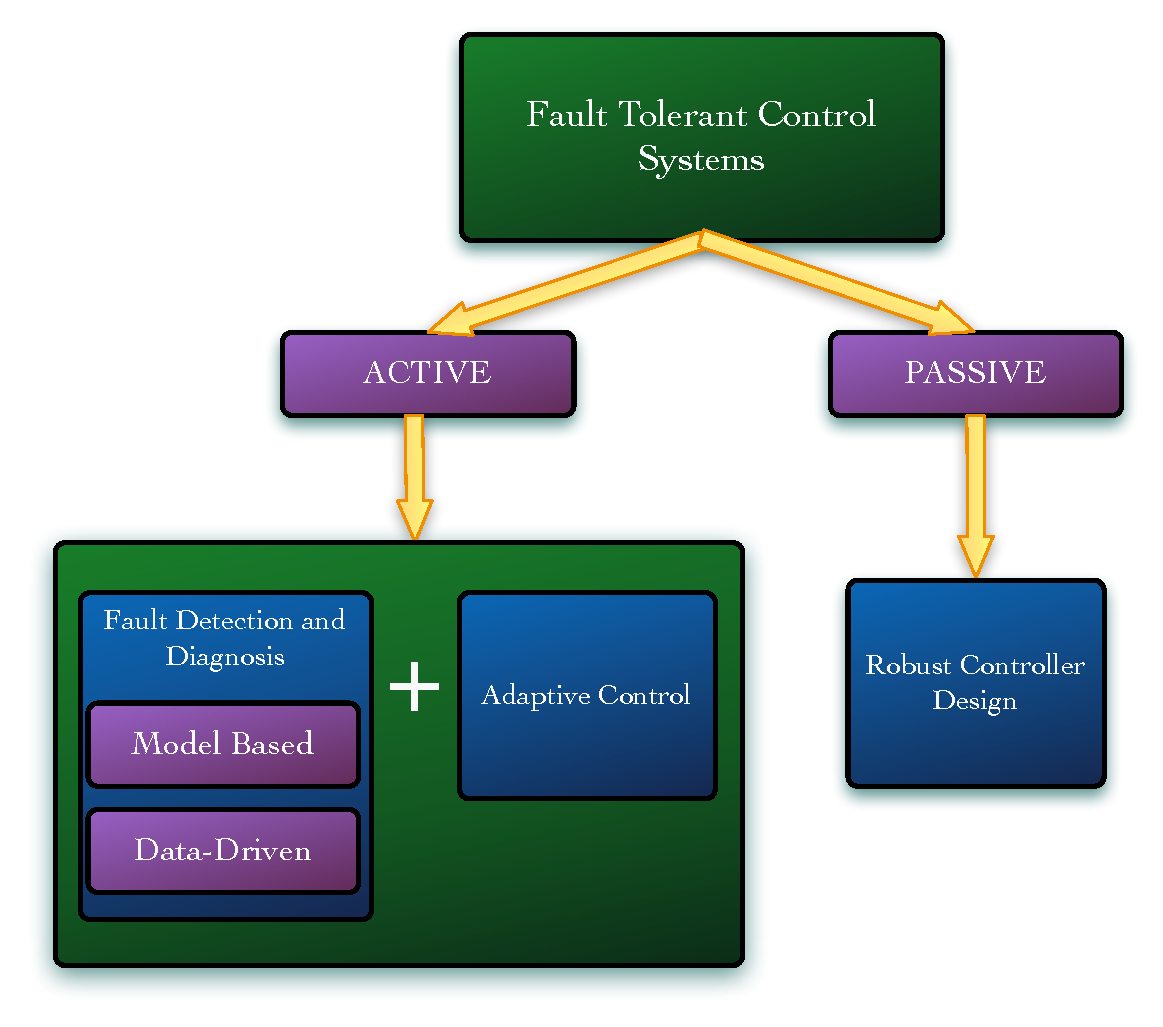
\includegraphics[width=11.3cm]{figures/FTCmethods}    % The printed column width is 8.4 cm.
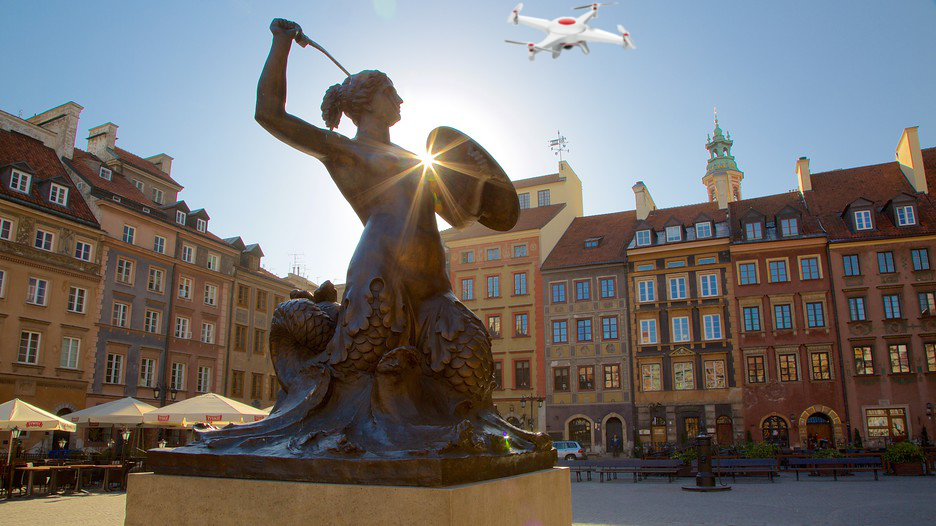
\includegraphics[width=11.3cm]{figures/mermaid_statue_drone}
\caption{Statue of mermaid in Riga handling airspace (for fun)} 
\label{fig:mermaid_statue_drone}
\end{center}
\end{figure}


While mentioning the efforts by different organizations to accommodate drones in airspace, we examine the present regulatory context from European and international perspectives.
The ICAO is a United Nations Organization working with 191 Member States of the Chicago Convention (Convention on International Civil Aviation) and global aviation organizations. 
At the present time, the international circulation of drones is not allowed by Article 8 of the Chicago Convention \cite{chicagoConvention}. 
Starting in 2003, the ICAO began a study on the Standards and Recommended Practices (SARPs) for drones, to which member states refer when developing their legally enforceable national civil aviation regulations. 
2018 is the proposed year for draft SARPs with a focus on international drone operations. 
Until then, the work of the ICAO can be traced by studies of the UAS Study Group (set up by ICAO in 2007), which developed the Circular 328 AN/190 on Unmanned Aircraft Systems \cite{ICAO_Circular}, an amendment to Annex 2 (Rules of the Air) \cite{amendment43toAnnex2} and Annex 7 (Aircraft Nationality and Registration Marks) \cite{amendment6toAnnex6}.
From a European perspective, Basic Regulation (Regulation EC No.216/2008) \cite{basicRegulation} is that which holds at present. 
Article 2 and Annex II limit the regulation to apply only to drones with a maximum take off mass above 150 kg and/or except operations on military, customs, police, firefighting, search and rescue, and experimental work. 
Those that are not covered by Basic Regulation are handled by national aviation legislation, which are not yet harmonized and mostly designed with an assumption that small drones are operating locally.
EASA is working on different aspects of drone integration into the airspace. 
Last year, EASA published the `Prototype' Commission Regulation on Unmanned Aircraft Operations \cite{prototypeRegulation}, after public consultancy with A-NPA 2015-10 (Advance Notice of Proposed Amendment) \cite{A_NPA_EASA2015}, and its resulting Opinion \cite{technicalOpinion} with an Explanatory Note of Opinion. 
Another work from EASA aims to authorize general principles for the \emph{type certification} for fixed wing and helicopter drones separately, using a policy adopted by the agency in 2009 (E.Y013-01) \cite{EY013_01policyStatementAirworthinessCertification}.

In the proposed regulation by EASA, an operation and risk centric categorization has been followed. 
\emph{Open}, \emph{specific}, and \emph{certified} are the three categories proposed, corresponding to the different risk levels that they entail.

\begin{itemize}
\item{\textbf{Open Category} encompasses low-risk operations, such as most leisure flights and some professional activities. 
Operations falling in this category do not require explicit authorization from civil aviation authorities. 
However, they are subject to strict operational limitations (e.g., no proximity to people, traffic, infrastructures; no dangerous items; one pilot per UAS; no item dropping). 
These operational limitations are sufficient to mitigate the low risk. 
Though some professional activities fit into this category, the main goal is to regulate leisure types of operation \cite{manfredi2018unmanned}.}
\item{\textbf{Specific Category} regroups medium-risk operations, such as operation beyond visual line of sight (i.e., no visual contact between pilot and UAV during flight). 
To facilitate the regulation process, several scenarios with specific operational limitations are designed. 
To operate within a scenario, the UAS needs to comply with a list of requirements.
For operations outside the scope of those scenarios, a risk analysis must be carried out to show that the existing risks are properly mitigated. 
To facilitate this risk analysis process, JARUS has developed a framework called the Specific Operations Risk Assessment (SORA). 
SORA considers threats --- which contribute to the risk --- and barriers --- which mitigate the risk --- in order to evaluate the actual risk of an operation, and decide if the resulting mitigated risk is low enough to allow the operation, as illustrated in Fig.~\ref{fig:sora_barriersReduced}.
The risk analysis needs to be validated by the authorities in order to authorize an operation not included in the standard scenarios \cite{manfredi2018unmanned}.}
\item{\textbf{Certified Category}  Operations with risk that cannot be mitigated in \emph{Specific Category} are evaluated in \emph{Certified Category}. 
These represent high-risk operations, such as a large cargo delivery in urban area. 
These are likely to be operations with a risk close to current manned aviation. 
As such, the aircraft, avionics, pilot/crew and operator will need to be certified in order to fly these operations. 
The fact that a certification process is involved increases the complexity of the introduction of UAS in these types of operations. 
Indeed,  
\begin{landscape}
\begin{figure}
\begin{center}
\includegraphics[width=24cm]{figures/sora_barriersReduced}    % The printed column width is 8.4 cm.
\caption{SORA structure: threats, threat barriers, hazard, harm barriers, harms} 
\label{fig:sora_barriersReduced}
\end{center}
\end{figure}
\end{landscape}

before being able to certify a piece of equipment, a standard must be developed for this equipment. 
Standardization can be best understood as the process of defining details and minimum requirements for safe and uniform operations across a diverse range of implementations. 
However, at present, not all of the parts required to fly a UAS have the corresponding standards, e.g., Detect And Avoid (DAA) systems, C2 links, pilot training. 
Thus, enabling this category of operation requires extra effort and time for the industry so as to agree on standards. 
For \emph{Certified Category}, harmonization at the ICAO is planned to allow international operations \cite{manfredi2018unmanned}.}
\end{itemize}

\begin{figure}
\begin{center}

\includegraphics[width=9cm]{figures/USpacePortable}    % The printed column width is 8.4 cm.
\caption{U-space illustration \cite{UTMairspace}} 
\label{fig:USpacePortable}
\end{center}
\end{figure}

Latest efforts for the integration of drones into airspace have welcomed a relatively new concept, called the `U-Space'. 
This approach has been adopted for immediate plans at the European level, to accommodate drones in urban areas. 
While EASA continues to search for solutions for the integration of drones in a variety of presumed airspaces, Commissioner Violeta Bulc has mentioned other pillars at a high level conference\footnote{Drones as a leverage for jobs and new business opportunities \cite{warsawDeclaration}} in Warsaw. 
She offers that in parallel to the efforts of EASA, there are two other pillars that need to be tackled; UTM (UAS Traffic Management) and the U-Space.
U-Space covers the usage of drones especially in `U-rban' areas with an equal share of airspace, in which case `\emph{U}' stands for `\emph{you}'.
To illustrate its availability to everyone, the services will be available through a mobile phone, as shown in Fig.~\ref{fig:USpacePortable}.
The goals are highly challenging \cite{UTMairspace}:

\begin{itemize}
\item{``Safe: safety at low altitude levels will be just as good as that for traditional manned aviation. The concept is to develop a system similar to that of Air Traffic Management for manned aviation.''}
\item{``Automated: the system will provide information for highly automated or autonomous drones to fly safely and avoid obstacles or collisions.''}
\item{``Up and running by 2019: for the basic services like registration, e-identification and geo-fencing. However, further U-Space services and their corresponding standards will need to be developed in the future.''}
\end{itemize}


\begin{figure}
\begin{center}
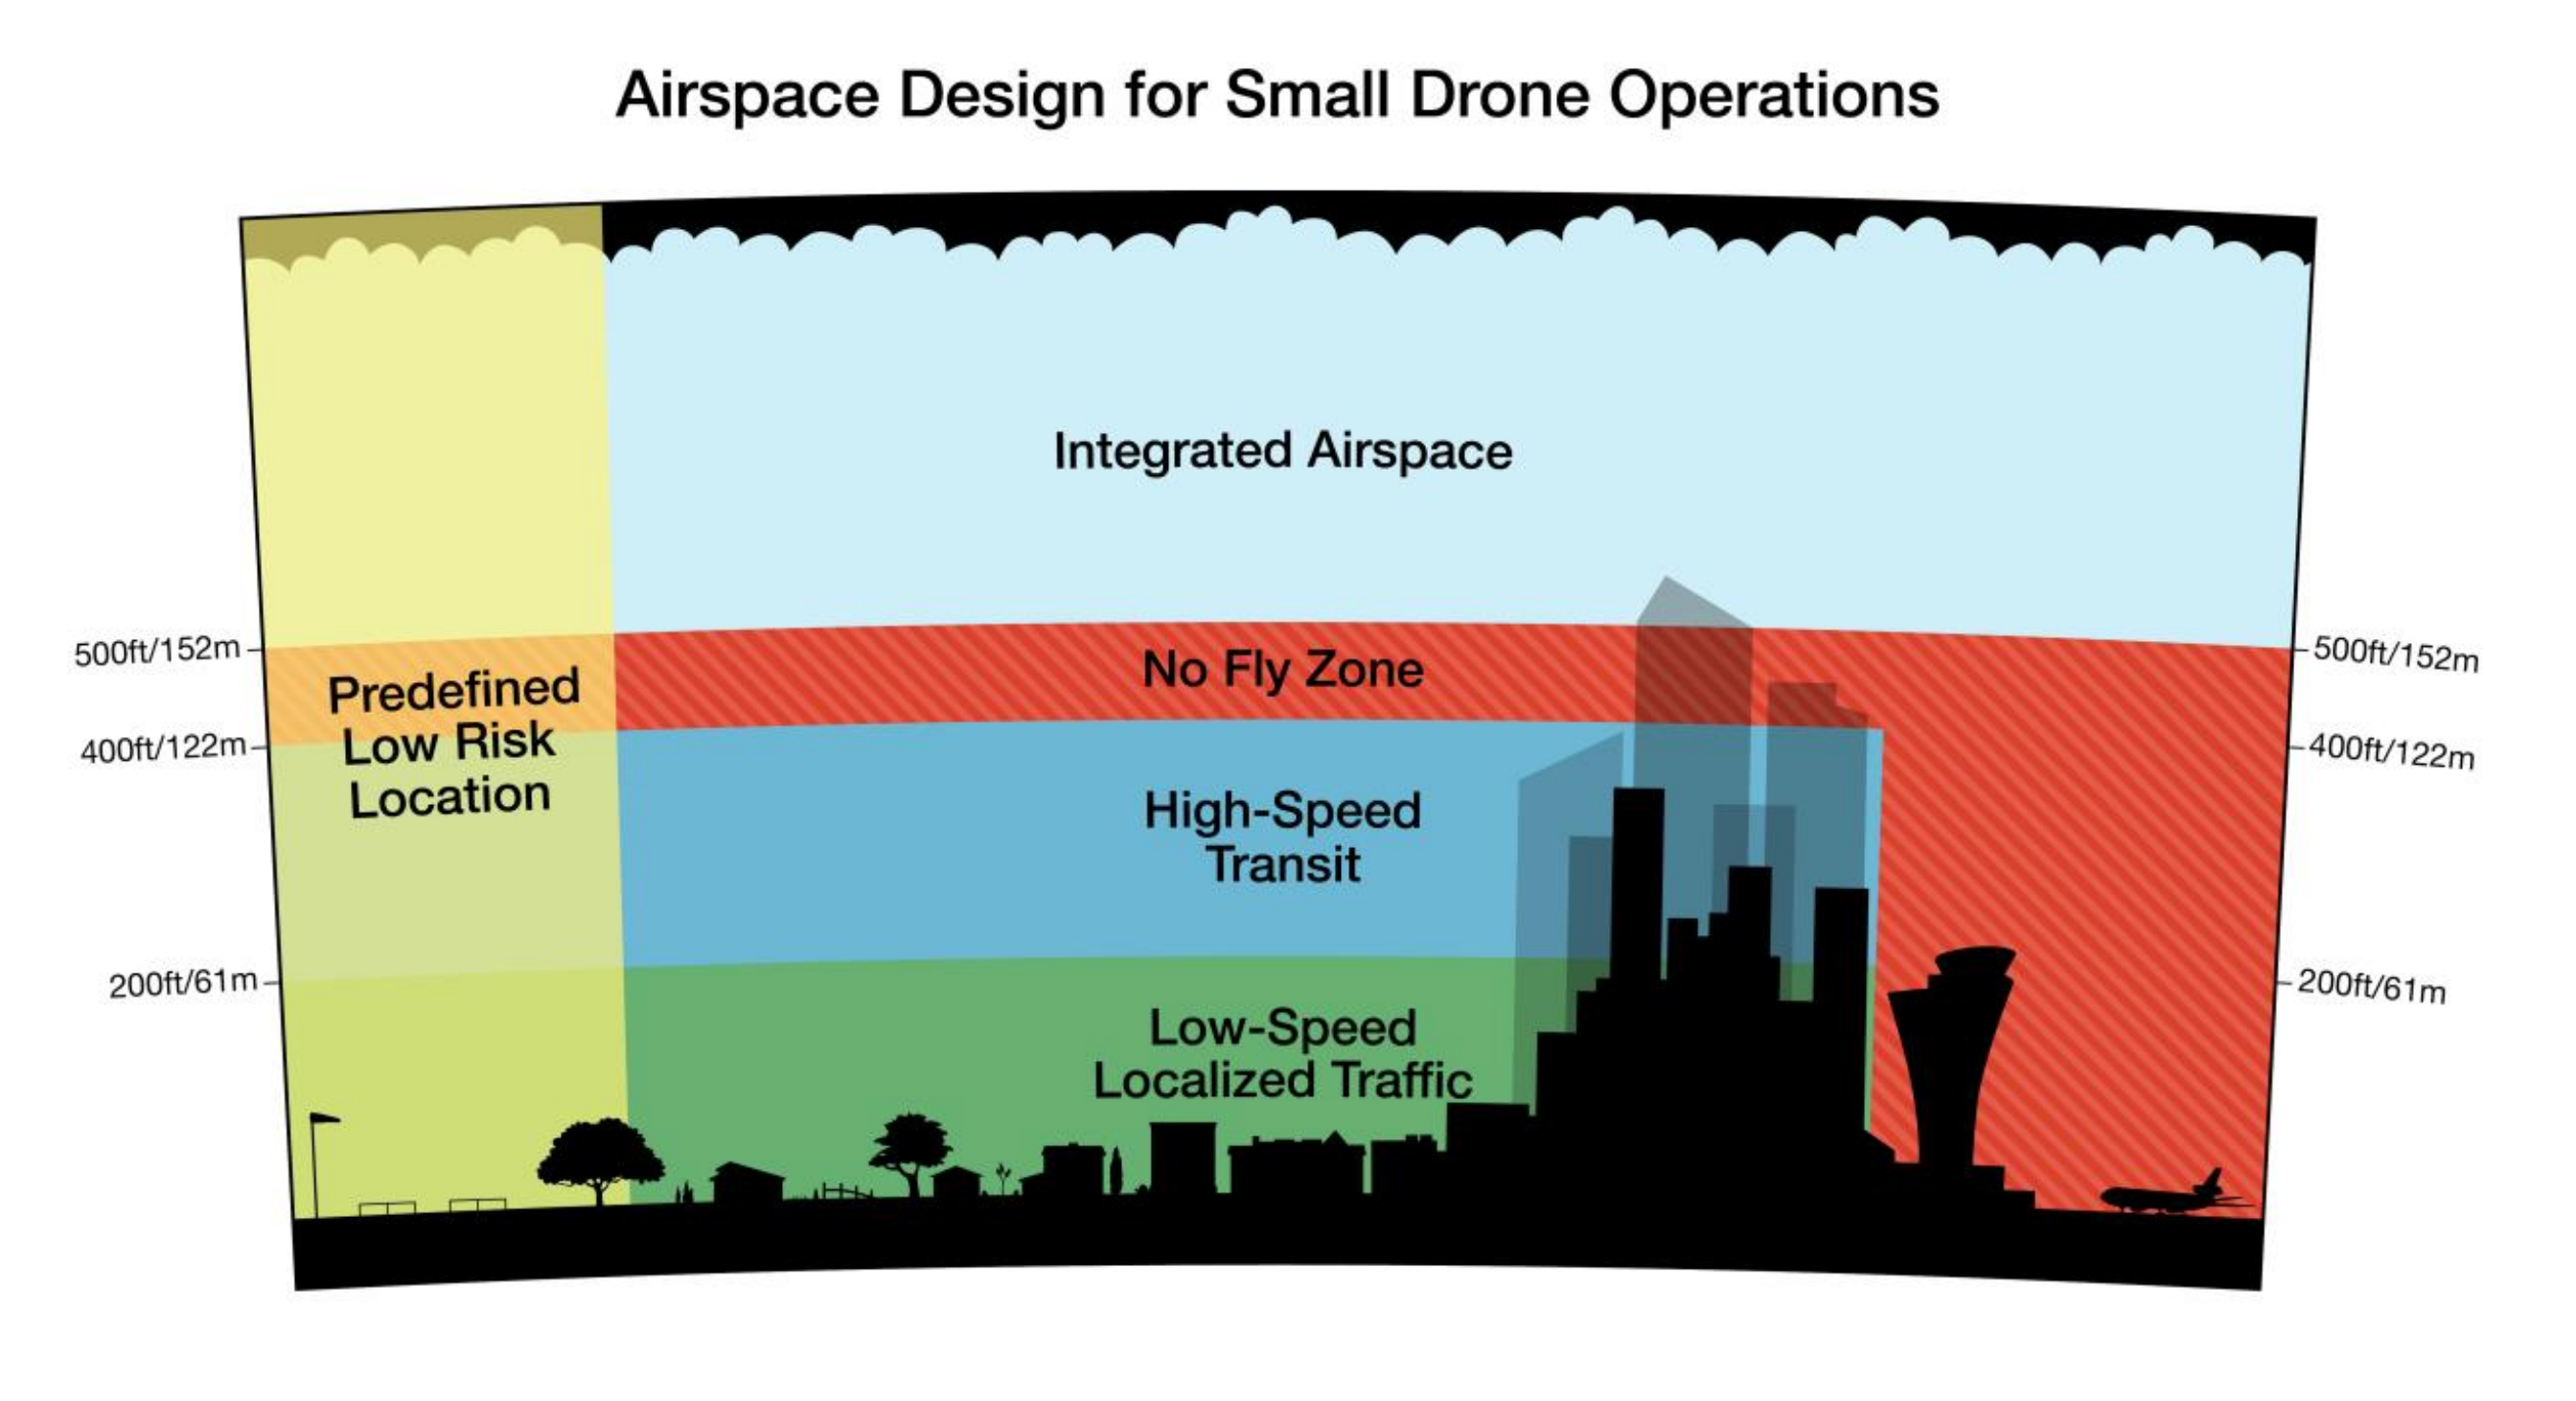
\includegraphics[width=17cm]{figures/amazonDroneOperations}    % The printed column width is 8.4 cm.
\caption{Airspace design for small drone operations by Amazon \cite{amazonAirspace}} 
\label{fig:amazonDroneOperations}
\end{center}
\end{figure}

EASA regulations already cover the airspace issued in U-Space, either under specific or certified categories (depending on the risk of the operation). 
Using U-Space, a faster integration is expected in urban areas.
We do not appear to be far from the images of flying vehicles populating the sky, as in science fiction --- but even more advanced --- without drivers, and more automated. 

In the US, in order to tackle the safety challenges and help the development of regulation, NASA is currently carrying out a four-year research program (up to 2019) to enable unmanned aircraft traffic management solutions which are structured and flexible when needed. 
To ensure safety, this integration needs to be achieved through airspace management and UAS reliability.
In addition, preliminary airspace designs, such as that proposed by Amazon shown in Fig.~\ref{fig:amazonDroneOperations}, identify different zones depending on the UAS capabilities, population density and altitude. 

United Arab Emirates (UAE) has accelerated the safe integration of drones into urban airspace, by settling an agreement for UAS Traffic Management (UTM) with Nokia, as part of its `Next generation network for mission-critical and smart city services' \cite{nokiaDubai}.
Aiming at tracking and managing all drones in the airspace, Nokia is offering solutions for automated flight permissions, no-fly zone regulation, beyond visual line of sight (BVLOS) safety operations utilizing LTE protocols for low latency, reliable and resilient communication. 
For compatibility with this system, drones will be equipped with LTE dongles and access modules for telemetry data access.



\iffalse
\subsection{Certification of analytical approaches NOT FINISHED }\label{ch2:certificationOfAnalyticalApproaches}

Due to the lack of the modeling for interaction in-between different FPE  (Flight Parameter Estimation), FDD and FTC modules in simulations, leaves them free from practical limitations, offering a long way to go for these analytical methods to be certified. 

[REF : certificationOfFDD]
[REF : clearanceOptimBased]


safety issues

http://www.techrepublic.com/article/12-drone-disasters-that-show-why-the-faa-hates-drones/

%FP7_RECONFIGURE REF : FP7RECONFIGUREgeneral page : 978 starting with 4 980 section 4. VERIFICATION AND VALIDATION

Regulations EU : https://easa.europa.eu/unmanned-aircraft-systems-uas-and-remotely-piloted-aircraft-systems-rpas

The increased cost will be inevitable for the demands of certification. REF : UAVreliabilityStudy

This increment could be even beyond expectations that it could lead to a cancellation of project:  REF : http://www.defenseindustrydaily.com/euro-hawk-program-cleared-for-takeoff-03051/

Regulations US : 

US Delivery Drones (News from Guardian http://www.theguardian.com/technology/2015/nov/06/alphabet-and-facebook-compete-with-secret-drone-plans)
--------------------
Even if the companies solve the technical challenges of keeping drones aloft for long periods, sharing data via lasers and serving city-sized areas, both Alphabet and Facebook still face regulatory hurdles. Neither company has been granted a waiver to the current FAA blanket ban on the commercial operation of unmanned aircraft.

Alphabet has applied for an exemption, called ?333? after a section of the FAA regulations, for its Project Wing delivery drones, but that is yet to be granted and in any case would only clear operation to a maximum height of 400ft. Google has also been testing its delivery drones in the US under a Certificate of Waiver or Authorization (COA) with Nasa, which permitted flights intended to help Nasa develop an automated air traffic control system for low-flying drones. This would not apply to drones flying far above other manned and unmanned aircraft.

?There?s not a lot to run into between 60,000 and 90,000 feet,? says Cummings. ?But I?m sure regulators would be deeply suspicious if Google and Facebook were flying these over the US.?

Facebook and Alphabet would not comment.

What's really standing in the way of drone delivery?
---------------------------------------------------------
http://www.theverge.com/2016/1/16/10777144/delivery-drones-regulations-safety-faa-autonomous-flight
\fi

\section{Paparazzi Autopilot System}
An open-source autopilot, \emph{Paparazzi} \cite{brisset2006paparazzi}, has been adapted to generate faulty control inputs during the flight. 
In this section, an introduction to \emph{Paparazzi} open-source autopilot system is given.
Next, we discuss the properties of open-source systems that would best serve the integration of drones into the airspace. 
To highlight the advantages of \emph{Paparazzi}, the best practices that are offered by EASA in its A-NPA \cite{A_NPA_EASA2015} are referred to, and the properties of \emph{Paparazzi} to achieve this are discussed.

\subsection{Open-source Autopilots for UAS}
With the new era of \gls{fpv} flights \cite{whatIsFPV}, especially for multi-rotor \gls{uav}s, there has been an exponential increase in the hardware and software of the open-source autopilots. A brief comparison of the popular current open-source and commercial autopilots is available in Table \ref{tab:autopilot_comparison}. Usually, the trend is to make the hardware as inexpensive as possible for recreational consumers. This reality is damaging to the reputation of open-source autopilots as they are considered as not reliable or robust, because they are being used without experience. Indeed, there exists a difference in the quality of sensors used in the open-source autopilot systems compared to commercial autopilots, and this is confirmed by the price of the units. This in turn makes a difference to the flight quality of the vehicles, however, with new on-board processing power, more complex estimation algorithms and filters are being used in order to overcome this problem \cite{baskaya2016flexible}.

\subsection{Introduction to \emph{Paparazzi Autopilot System}}

The \emph{Paparazzi} Autopilot System provides a software and hardware solution for low-cost mini and micro unmanned air vehicles. 
A fleet of \emph{Paparazzi} equipped drones can be seen in Fig.~\ref{fig:ENACdroneFleet}.

This began as a personal project in 2003 by Pascal Brisset and Antoine Drouin, and afterwards gained the support of ENAC in 2005. 
Being one of the first (if not \emph{the} first) open-source autopilot system in the world, \emph{Paparazzi} has attracted much attention, and has led others to start new branches and systems. % This phrase may need some proof actually, but it is hard to find anything officially...
The software is originally packaged for Debian/Ubuntu but can be manually installed on any GNU/Linux operating system, even including MacOS-X. 
However, it is not compatible with Windows which automatically eliminates $90\,\%$ of the possible user community, and therefore it is not as popular as other existing autopilot systems currently on the user market.


\begin{landscape}
\begin{table*}[t]
	\caption{Comparison of popular open-source and commercial autopilots \cite{baskaya2016flexible}.}
	\centering
	\begin{tabular}{lcc >{\centering}m{1.2cm} >{\centering}m{1.8cm} cc >{\centering}m{1.3cm} >{\centering}m{1.1cm}}
		\hline
		Open-Source & Vehicle type & Hardware & Multi UAV & Flight Plan & Path Definition  & Geofencing & Collision Avoidance & Latest stable release		\tabularnewline	
		% & & & & & & & & release\\
		\tabularnewline
		\hline
		Paparazzi  & Fully configurable        & varied   & yes   & scriptable & Formula Based          & 3-D  & UAV TCAS & 21-06-16\tabularnewline
				& & & & & & & &  \tabularnewline
		PixHawk    & Fully configurable        & specific & yes   & scriptable & Circles Lines Patterns & 3-D  & none     & 06-08-16\tabularnewline	
				& & & & & & & &  \tabularnewline
		Ardupilot  & Copter Plane Rover        & varied   & alpha & scriptable & Circles Lines Patterns & 2-D  & none     & 22-06-16\tabularnewline	
				& & & & & & & &  \tabularnewline
		OpenPilot  & multicopter               & specific & none  & NA         & NA                     & none & none     & 15-05-15\tabularnewline	
				& & & & & & & &  \tabularnewline
		AeroQuad   & multicopter               & varied   & none  & NA         & NA                     & none & none     & 31-01-13\tabularnewline	
		\tabularnewline	
		\hline
		Commercial & & & & & & & &  		\tabularnewline	
%				   & & & & & & & &  		\tabularnewline	
		\hline
		Picollo    & Copter Plane              & specific & none  & dynamic    & Way Point              & NC   & NC       & NC   	\tabularnewline	
				& & & & & & & &  \tabularnewline
		MicroPilot & Copter Plane Rover Blimp  & specific & yes   & dynamic    & Way Point              & NC   & NC       & NC   	\tabularnewline	
				& & & & & & & &  \tabularnewline
	\end{tabular}
	\label{tab:autopilot_comparison}
\end{table*}
\end{landscape}

\begin{figure}[!hbt]
\begin{center}
%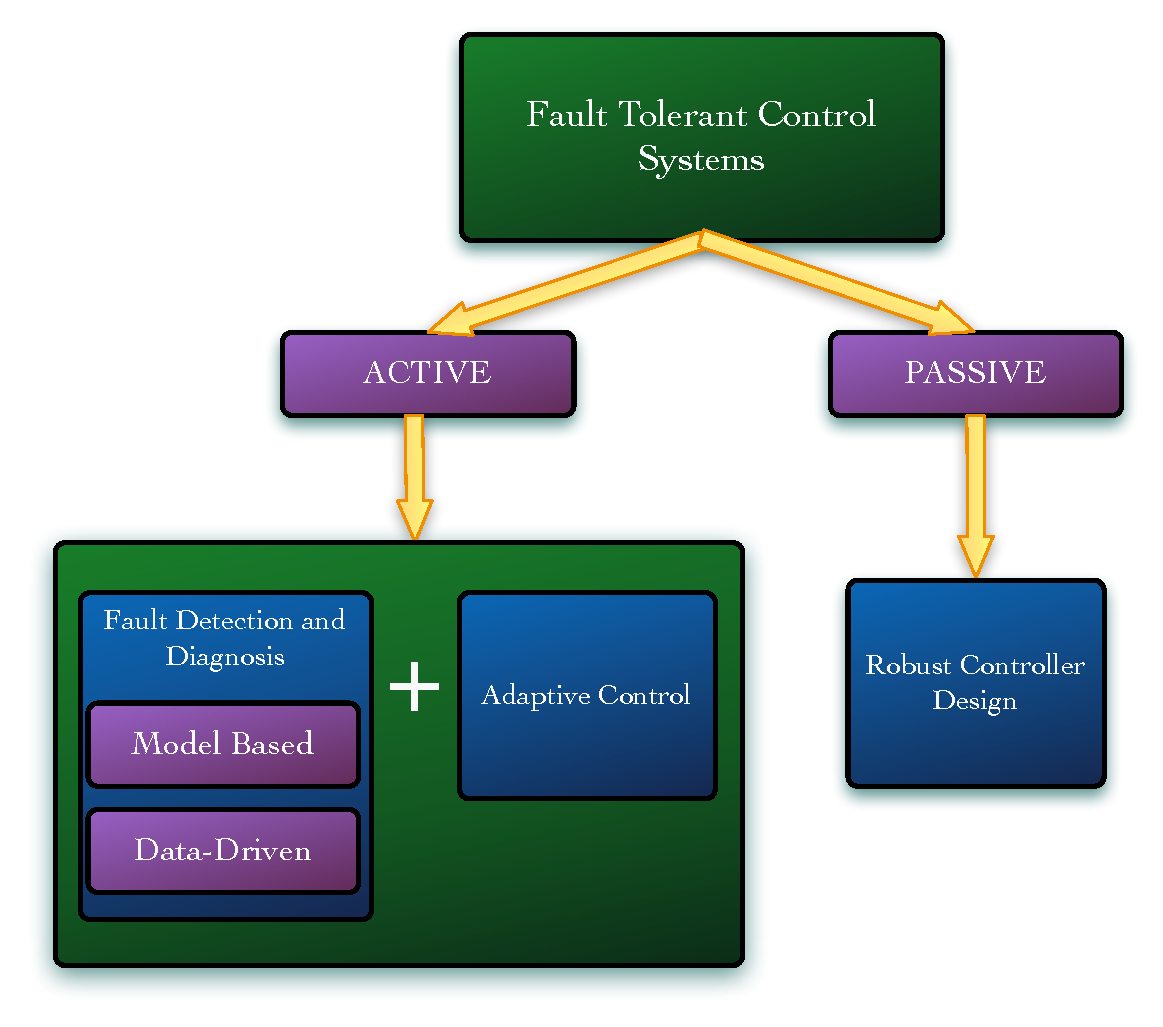
\includegraphics[width=11.3cm]{figures/FTCmethods}    % The printed column width is 8.4 cm.
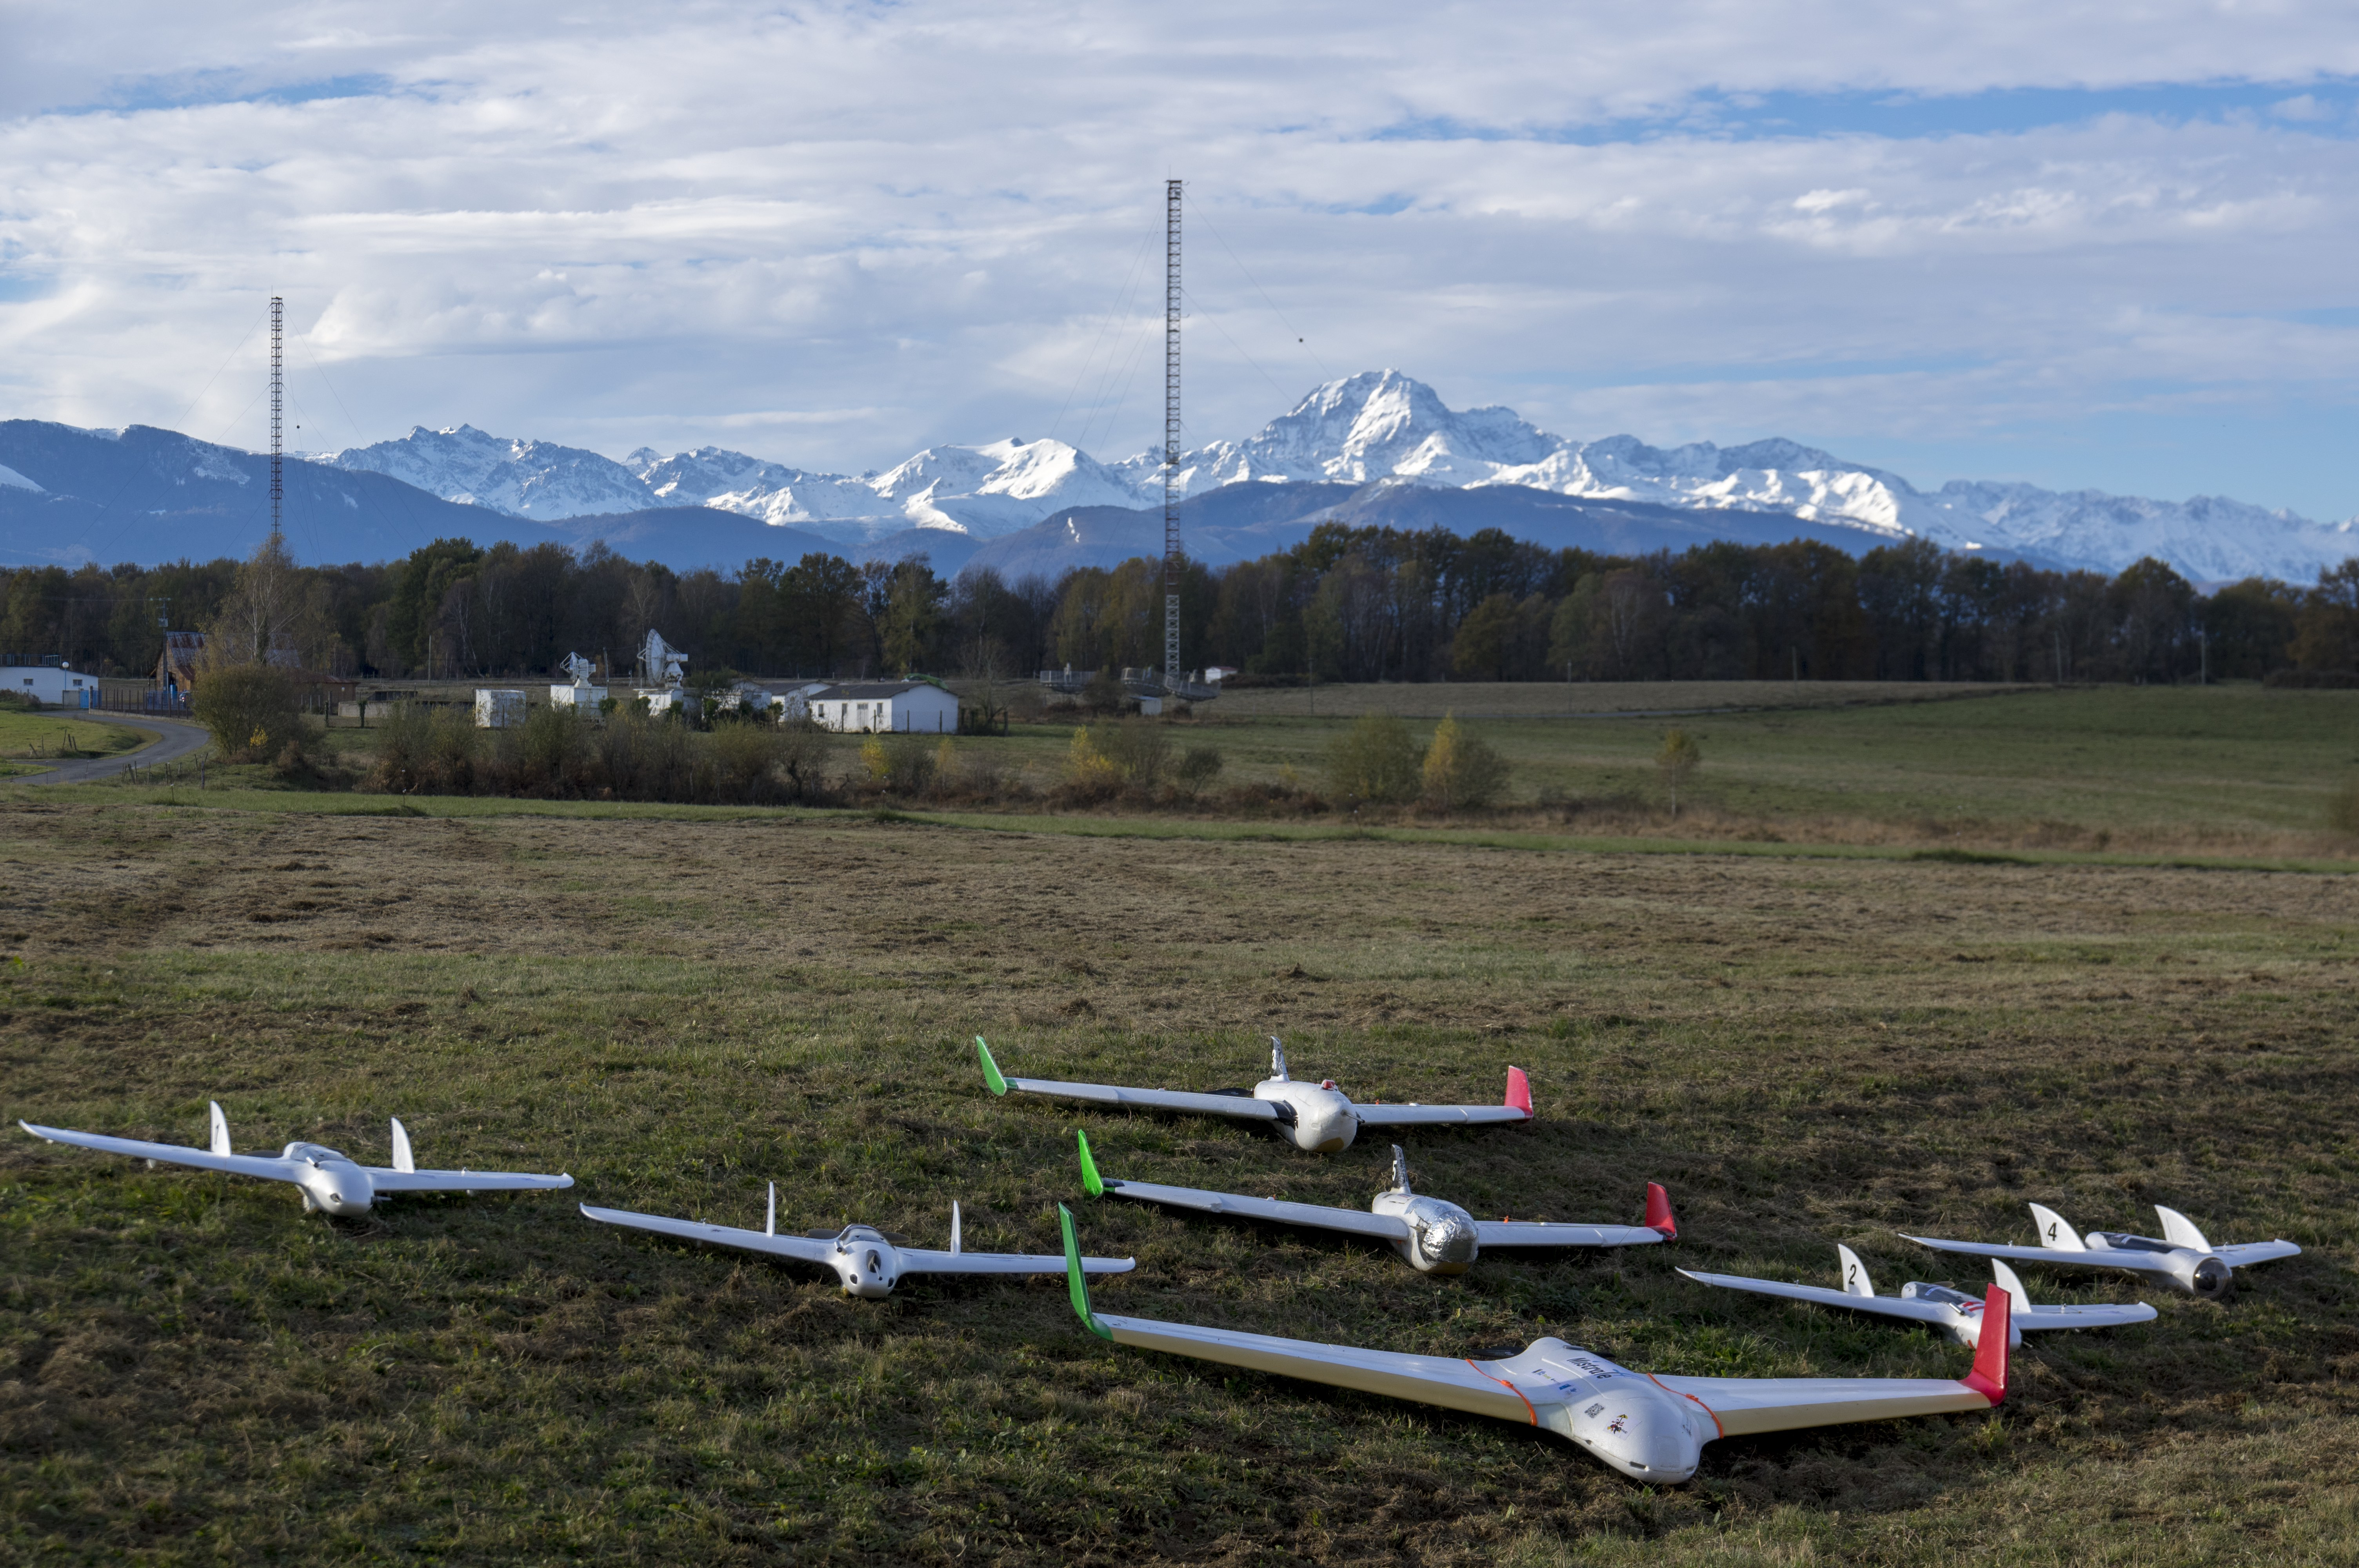
\includegraphics[width=13.3cm]{figures/ENACdroneFleet}
\caption{Fleet of \emph{Paparazzi} equipped drones from ENAC UAV laboratory in a flight campaign with the \emph{Pyrenees} in the background. Photo by Alexandre Bustico.} 
\label{fig:ENACdroneFleet}
\end{center}
\end{figure}


\begin{figure}[!hbt]
\begin{center}
%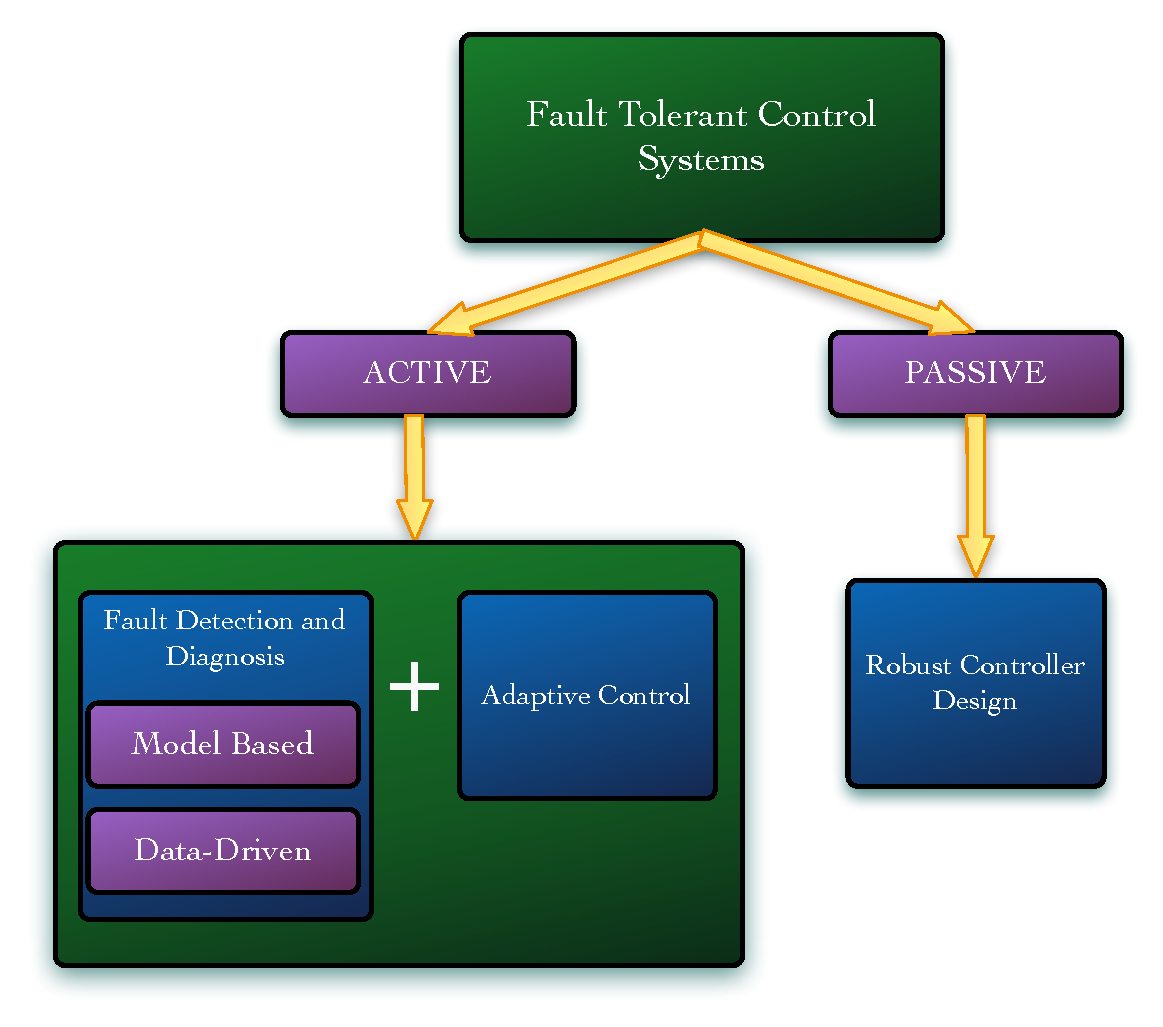
\includegraphics[width=11.3cm]{figures/FTCmethods}    % The printed column width is 8.4 cm.
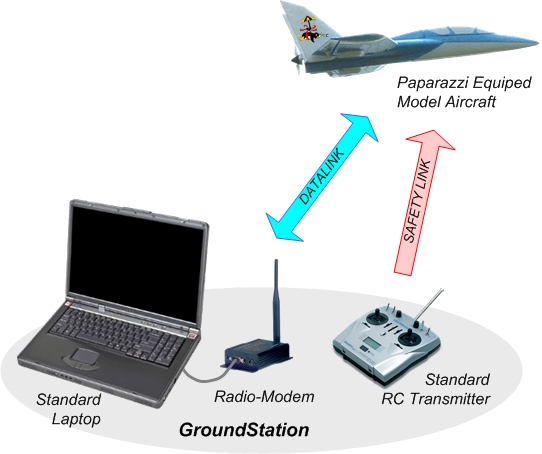
\includegraphics[width=11.3cm]{figures/Paparazzi_System_overview}
\caption{Paparazzi Autopilot System overview} 
\label{fig:Paparazzi_System_overview}
\end{center}
\end{figure}


Being one of the first open-source autopilot systems in the world, \emph{Paparazzi} covers all three segments: ground, airborne, and the communication link between them, as shown in Fig.~\ref{fig:Paparazzi_System_overview}. 
The ground software of \emph{Paparazzi} is mainly written in Ocaml, with some additional parts in Python and C. 
Thanks to its middle-ware communication bridge called Ivy-Bus, external software can be directly connected with the publish and subscribe method to the ground segment, without needing to modify on code.
Airborne software is written in C, however there is an on-going effort to support C++ \cite{baskaya2016flexible}.

One of the distinguishing features of \emph{Paparazzi} is to support multi-UAV flights (Figure~\ref{fig:pic2}). Several projects have been using \emph{Paparazzi} Autopilot System because of this additional feature. The communication with each vehicle is established by the ground control station, however air-to-air communication between flying vehicles and the internal relay of information to the ground control station is being implemented (for a future version).

\begin{figure}
	\centering
	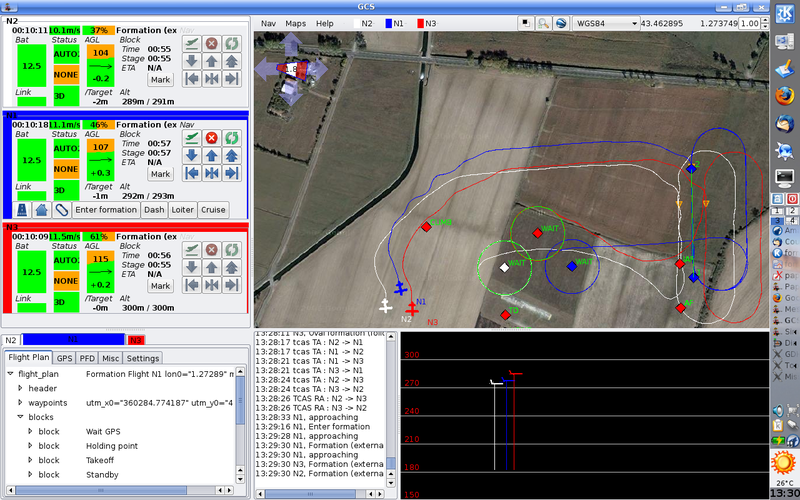
\includegraphics[width=1\textwidth]{figures/pic2}
	\caption{Ground Control Station showing trajectories of 2 \gls{uav}s using the \gls{tcas} system}
	\label{fig:pic2}
\end{figure}

\emph{Modules} are the easiest and most flexible way of adding new code into \emph{Paparazzi}. 
There are over $130$ modules written for \emph{Paparazzi} by several developers and researchers, including meteorology, imagery, surveillance, advance navigation, formation flight, and collision avoidance, etc. 
A photo taken during a \emph{Paparazzi} mission in a campaign for meteorological studies by \emph{MeteoFrance} is provided in Fig.~\ref{fig:snowWhite}. 
MeteoFrance is French national meteorological service, and uses drones as tools to conduct research for meteorological studies.

\begin{figure}
\begin{center}
%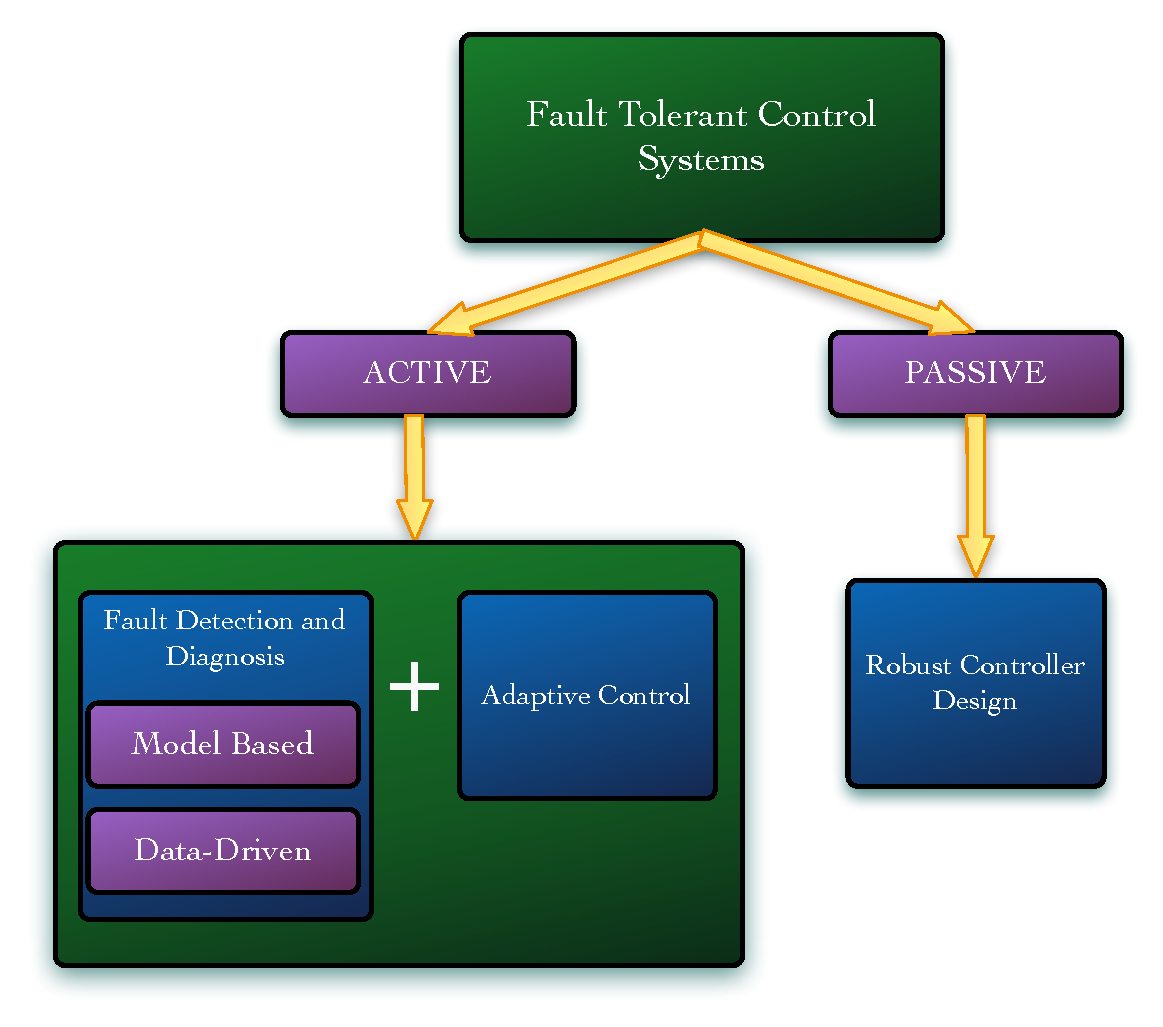
\includegraphics[width=11.3cm]{figures/FTCmethods}    % The printed column width is 8.4 cm.
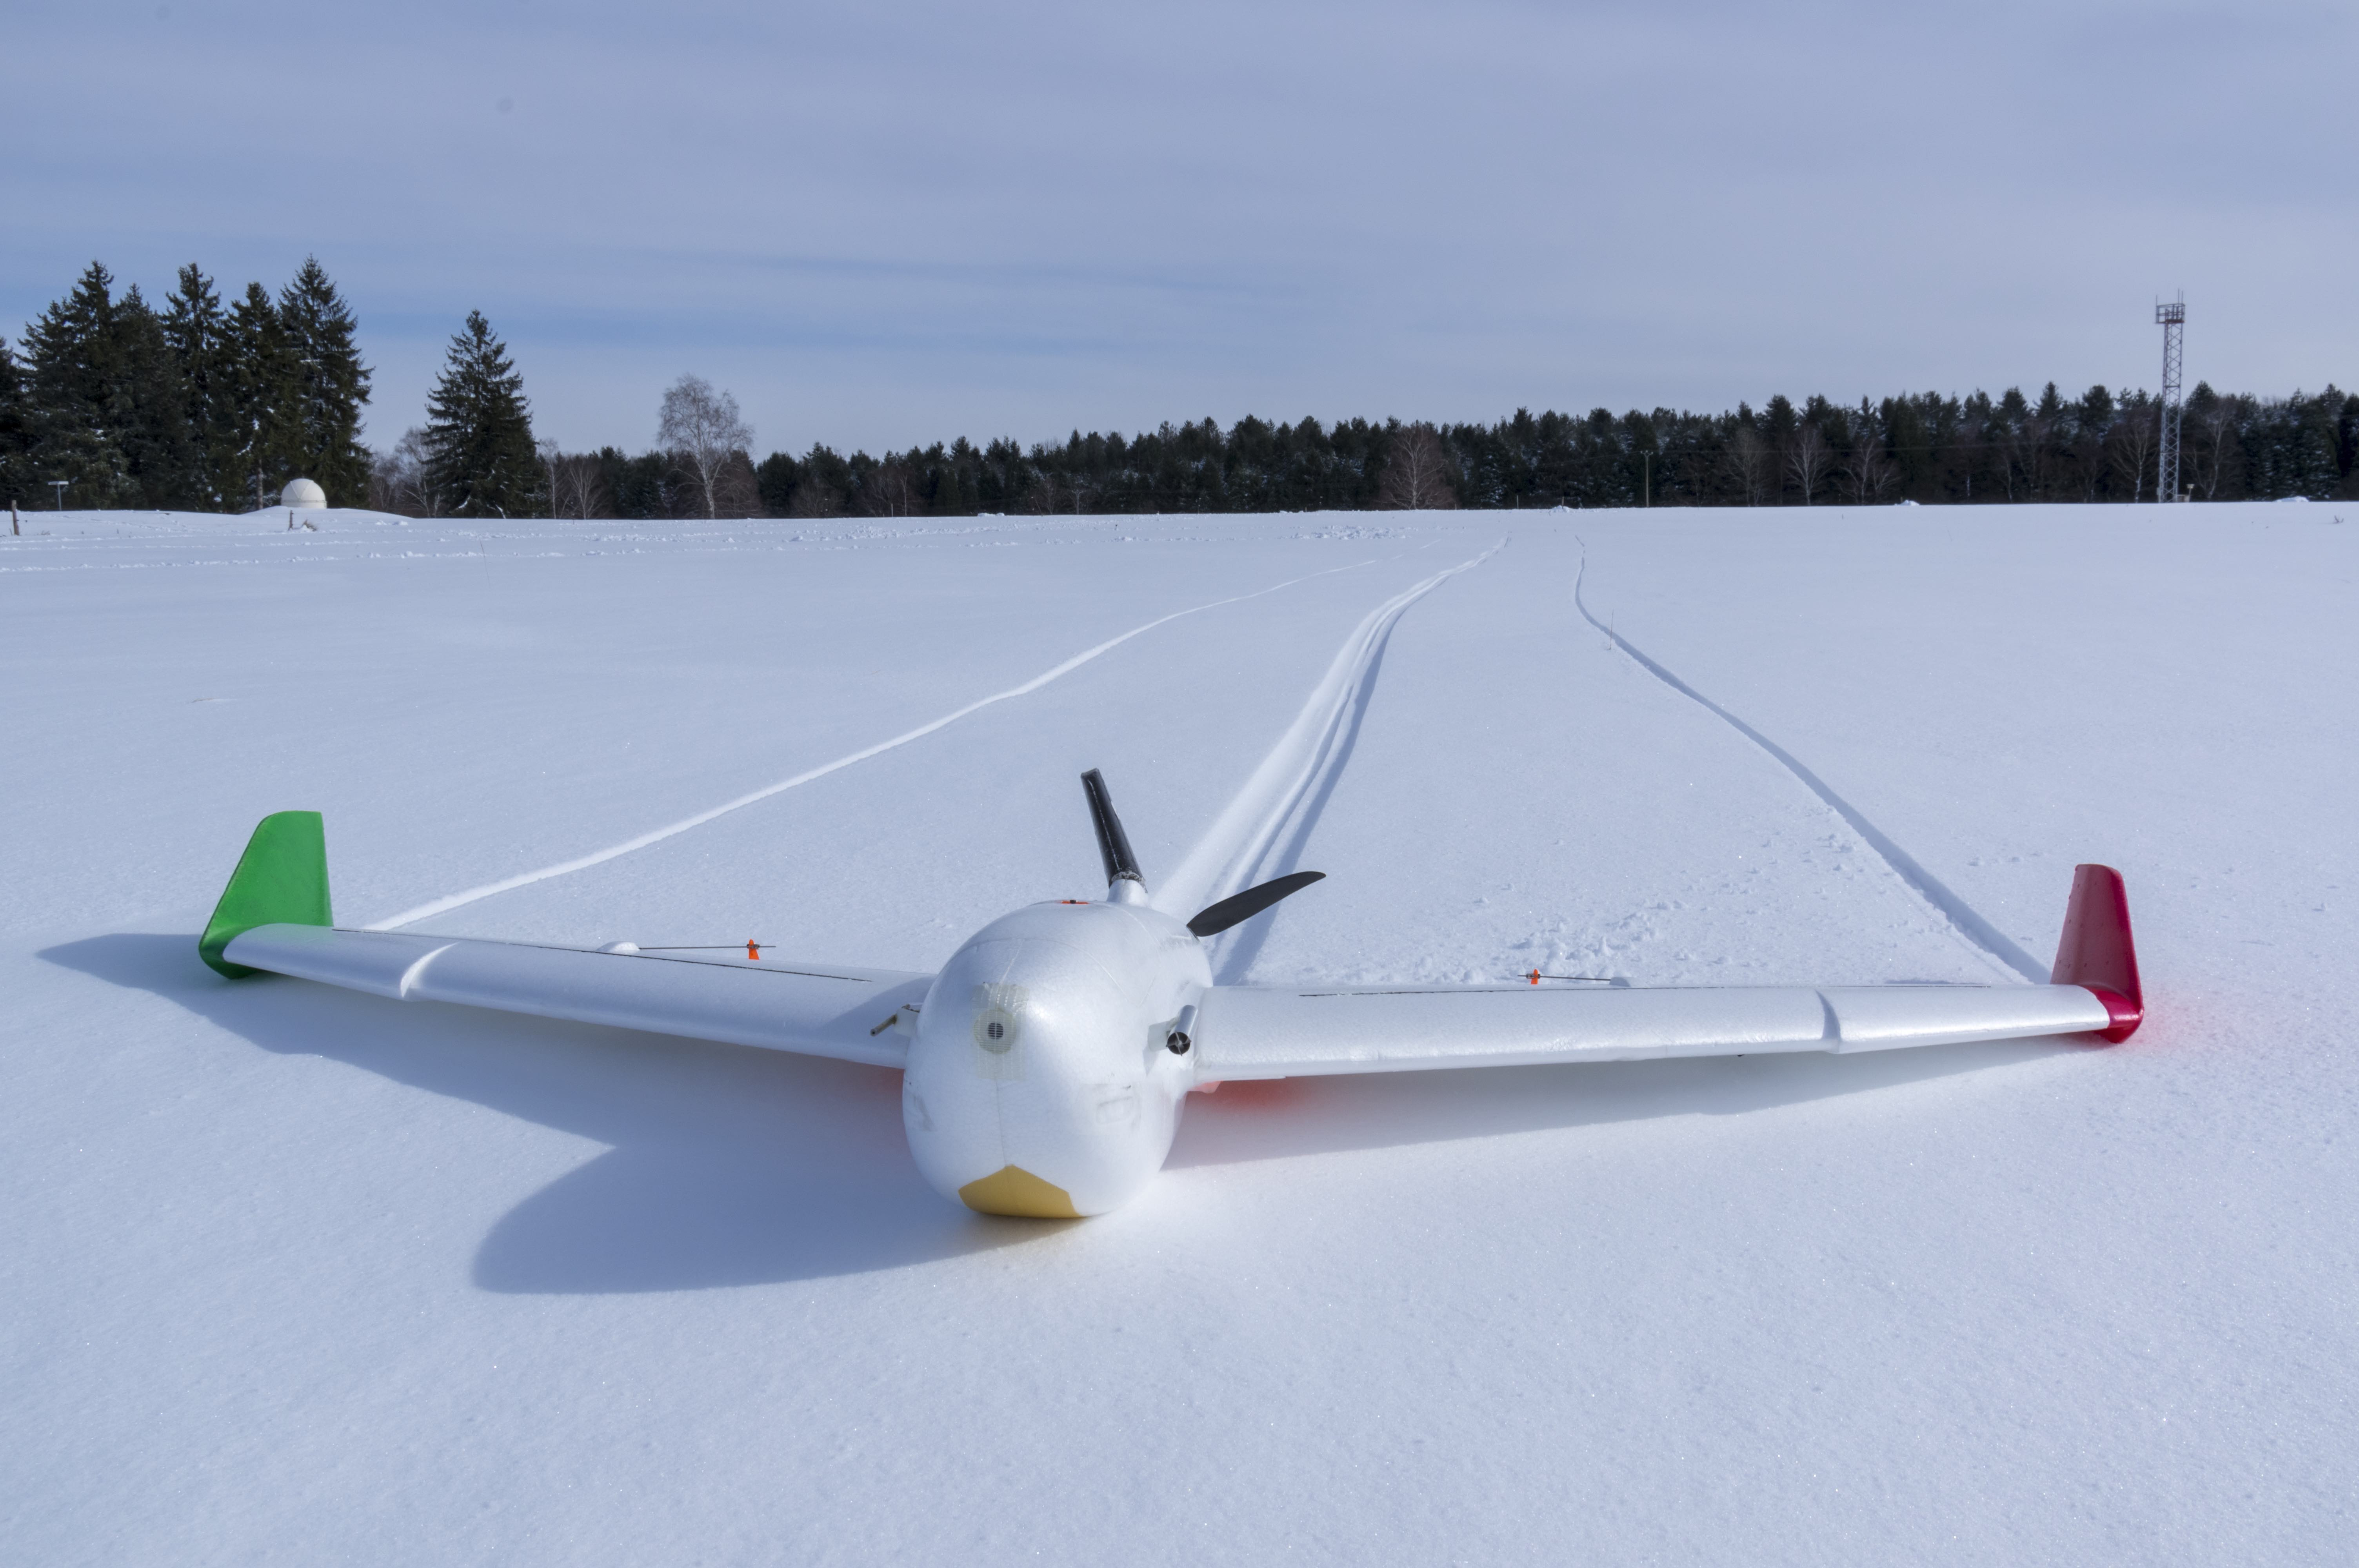
\includegraphics[width=13cm]{figures/snowWhiteJPG}
\caption{Drone equipped with \emph{Paparazzi} on a mission for meteorological studies by \emph{Meteofrance}. Photo taken by Alexandre Bustico.} 
\label{fig:snowWhite}
\end{center}
\end{figure}


\emph{Paparazzi} has its own complete flight plan language, where the user can define any possible trajectory using existing commands, such as circle, line, hippodrome, figure-eight, survey, etc. 
Additionally, any function written in C language can be called from the flight plan and executed. 
This opens up a lot of application possibilities, such as triggering a navigation procedure via a sensor output.

A real-time operating system based on ChibiOS has been used since 2015. 
The first implementation was mainly for adding a separate thread in order to make on-board logging at a high frequency. 
On going work is to divide all autopilot tasks into individual threads and manage everything according to priorities which will increase the safety and reliability.
%Priorities can be handled over different tasks in order to increase the safety and reliability.

There exists over 20 different autopilot boards capable of running \emph{Paparazzi}. Additionally, several mission-based custom sensor boards have been designed under the \emph{Paparazzi} project, such as \emph{Meteo-Stick}\footnote{http://wiki.paparazziuav.org/wiki/MeteoStick\_v1.10}. 
In this thesis, flights have been realized with an \emph{Apogee}\footnote{https://wiki.paparazziuav.org/wiki/Apogee/v1.00} which is shown in Fig.~\ref{fig:apogeePaparazzi}.

\begin{figure}
\begin{center}
%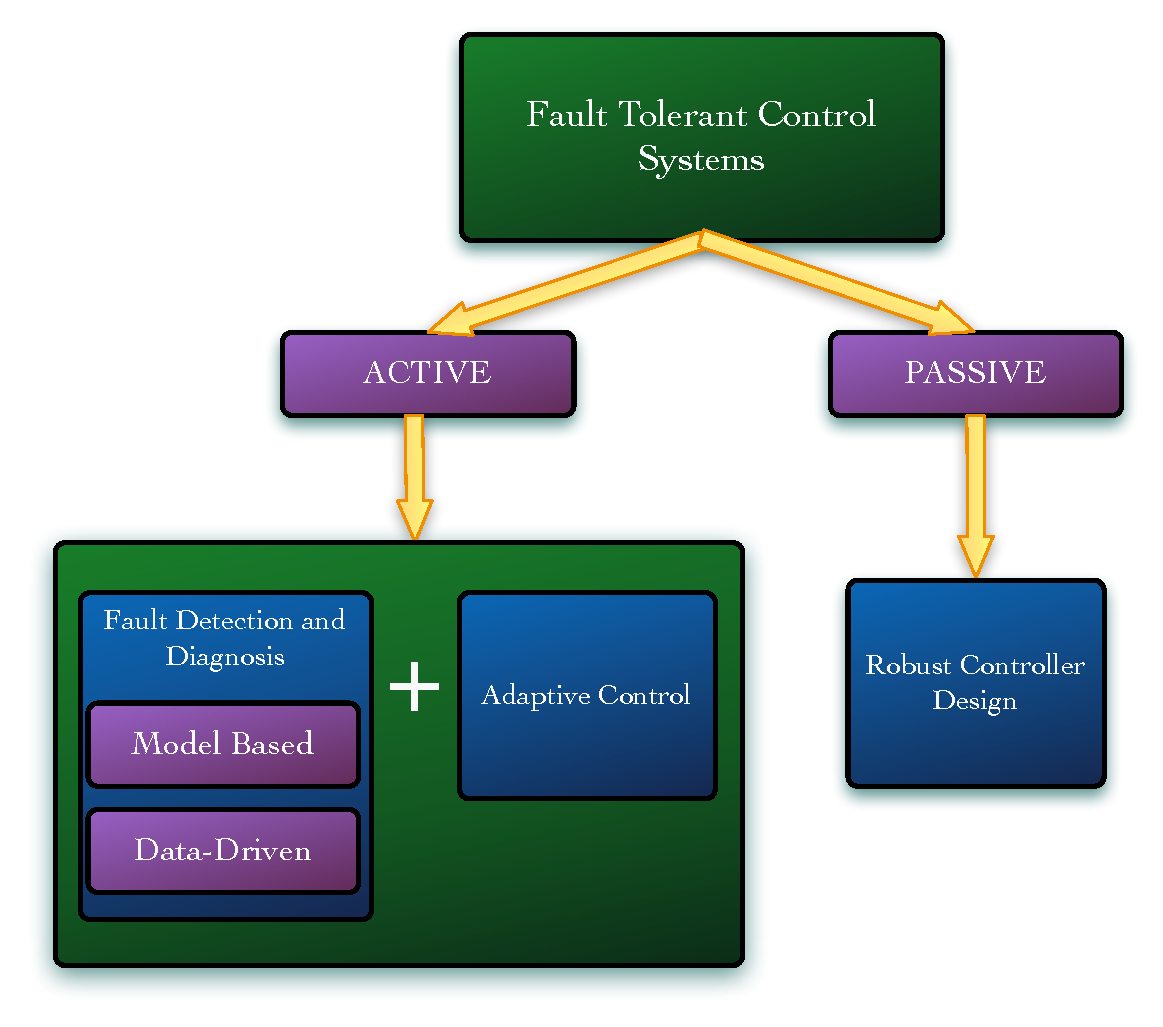
\includegraphics[width=11.3cm]{figures/FTCmethods}    % The printed column width is 8.4 cm.
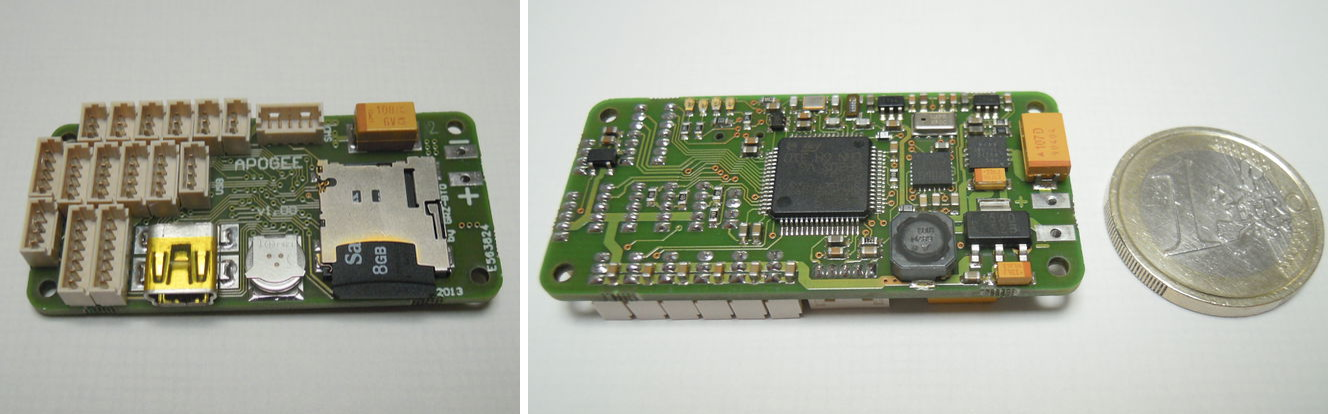
\includegraphics[width=14cm]{figures/apogeePaparazzi}
\caption{Front and back view of \emph{Apogee} autopilot} 
\label{fig:apogeePaparazzi}
\end{center}
\end{figure}

For the faulty flight data gathering necessary for this thesis, some modifications to the \emph{Paparazzi} autopilot were necessary: first, injecting the real-time faults from GCS; and  second, editing the controller on board so that the sent faulty input values configure the servos when changed from the GCS. 

The rest of this section highlights the capacity of \emph{Paparazzi} capacity to tackle issues encountered during the integration of \gls{uas}s into the airspace. These issues have been grouped into three categories: modularity, congestion management and reliability. For each category, \emph{Paparazzi} offers a unique set of features to deal with these issues.

\subsection{Open-Source Systems in Relation to the New Regulatory Context}

In this section, we present the \emph{Paparazzi} open-source auto-pilot system and its features, as a tool towards the safe integration of low altitude UAS into the National Air Space (NAS). 
\emph{Paparazzi} is favored thanks to its modular design, its support for congestion management and evolving reliability.
We believe that the flexibility required for such solutions calls for open architecture. To ensure safety, this integration needs to be achieved through airspace management and UAS reliability.
Preliminary airspace designs (for example, Amazon's design) identify different zones depending on the UAS capabilities, population density and altitude. 
Furthermore, the evolution of national rules increases the push to cope variety of requirements. Open-source and modular architectures are keys to successfully adapting to these requirements. 
From UTM point of view, \emph{Paparazzi} provides features to ease congestion management, such as dynamic geofencing, trajectory communication and collision avoidance. 
Concerning reliability, current regulations focus on flight constraints but may be expected to involve regulations on software and hardware components as well. 
In such a case, the increased cost will be inevitable for the demands of certification. 
In the \emph{Paparazzi} software case, parts of the code have been formally proved and stable versions have thousands of flight hours. Such heritage may ease the certification process for smaller companies.
In addition to its flexibility and reliability, \emph{Paparazzi} offers a unique set of features as an open-source software, so as to achieve safe integration of low altitude UAS into the airspace.

% More specifically, this paper shows how the use of the Paparazzi open source auto-pilot system can ease the integration of low altitude UAS. 

\subsection{Modularity}
The current evolving nature of regulations, and the variety of organizations in charge of the airspace rules, demands flexible solutions to cope with this unique environments. \emph{Paparazzi}, as an open-source autopilot system, is easily modifiable through its modules to be able to offer such flexible solutions.  

\subsubsection{Airspace Categorization}
The \gls{uas} in the \gls{nas} project points to a performance-based routine access to all segments of the national airspace for all unmanned aircraft system classes, after the safety and technical issues are addressed thoroughly. 
Initially, \gls{nasa} and \gls{faa} seem to have a short-term goal to integrate \gls{uas} in low-altitude airspace as quickly as possible. 
They further aim to accommodate increased demand safely and efficiently in the long term. \gls{nasa} and \gls{faa} appear to manage the airspace above 500 feet and that below separately. \gls{easa}, tasked by the European Union, is planning a risk-based approach, accommodating the \gls{uas} in the airspace under three different categories: low risk; specific; and high risk \cite{A_NPA_EASA2015}. Both regulators seem to categorize the airspace and scale regulatory needs according to certain criteria. To respond to the different needs of the different categories, flexibility given by the high level of modularity of open-source autopilot systems will be critical. 
Customizability of the software and hardware depending on the airspace gives a chance for the larger airspace community to utilize \emph{Paparazzi}, scaled for their specific needs. A larger community using the same system would lead to a natural evolution of the system towards a better design.

\subsubsection{National Regulations}
International \gls{uas} flight is somewhat hampered by the Chicago convention unless an agreement holds between Contracting States \cite{A_NPA_EASA2015}. The \gls{icao} is aiming to develop international standards and recommended practices to which the member states can refer when developing their national civil aviation regulations. Although member states are planning to refer to the same standards and national aviation legislations, those will not be exactly the same because of the different expectations of nations towards \gls{uas} aviation. Thanks to the modular nature of the \emph{Paparazzi} software and hardware suite, the functionality of the system could be enhanced according to the specific regulations held in the area of utilization.

\subsubsection{Accommodating evolution of regulations}
Prescriptive rules seem to cause some difficulties since the technical area of the \gls{uas} systems develops rapidly \cite{A_NPA_EASA2015}. Innovations, both on the aircraft and on the type of operation of the \gls{uas}, will accelerate especially after the regulations are set. Thus, regulatory bodies call for refinable operational requirements and systems architecture to evolve into a safer and more efficient integration of \gls{uas} into the airspace. The systems to cope with the regulations should also be modular and flexible in order to not be superseded by innovations in the area. 
Thus, the aviation regulatory bodies aim to achieve designs with flexibility where possible, and structure where needed. Having flexible hardware and software increases modularity, which is for the most part supported via open-source systems.

\subsection{Congestion Management}
According to \textit{UAV Factory}, one of the large European \gls{uas} companies, ``The future of the UAV industry is likely to be shaped by airspace congestion'' \cite{europe_report_civilian_drone}.
	Indeed, high level airspaces are becoming crowded, and large-scale solutions, such as NextGen (US) or SESAR-JU (EU), are necessary to increase airspace capacity while maintaining the current safety levels.
	However, there is no such existing management solution for \gls{vll}. Yet, large projects like Amazon's Prime Air and Google's Project Wing are already ready to populate the \gls{vll} airspace.	
	
	Part of the congestion management problem is to avoid conflicts (and more importantly, collisions), between the \gls{uas} through strategic deconfliction and safety nets.
	Another purpose of the congestion management system is to make sure that \gls{uas} do not go where they are not supposed to go, thus requiring geofencing.
	In order to implement the previously mentioned systems, the \gls{uas} autopilot needs to be able to perform complex operations, for example, static waypoints following is likely to be insufficient.
	In the following, we divide these issues into four topics of interest: 4-D trajectory management; geofencing; safety nets; and complex operations, and show how the \emph{Paparazzi} system addresses them.
	
	\subsubsection{4-D Trajectory Management}
		As noted in \cite{erzberger_4D_2002}, 4-D trajectories will be central in future airspace management methods. The principle of 4-D trajectory management is to have every \gls{uas} broadcasting its trajectory up to some time horizon and receive \gls{utm}'s clearances under the form of trajectories. 
		The trajectory information contains a path, the series of points through which the \gls{uas} will pass, and times associated to each of these points. 
		Thanks to this information, the idea is to perform pro-active deconfliction, as explained by Thomas et al. in \cite{thomas_4D_2015}. It implies that \gls{utm} detects future conflicts along the trajectories of all \gls{uas} and deconflicting them as safely and early as possible.
		This kind of approach requires the autopilot to represent \gls{uas} motions with trajectories and to be able to transmit them, which is the case in \emph{Paparazzi}.
		
		\emph{Paparazzi} originally supports a basic description of trajectories based on circles and straight lines, but recent updates allow it to process advanced trajectories as well. 
		Indeed, \emph{Paparazzi} can represent trajectories as functions in 2-D (x, y), 3-D (x, y, z) or 4-D (x, y, z, t). The only requirement is for the function to be differentiable at least two times at every point. The function and its derivatives closed forms are computed offline and can then be quickly evaluated online.
		Moreover, gains can be tuned to adjust the convergence speed from the \gls{uas} starting point to the given trajectory. These gains influence the convergence path to a given trajectory and the resulting trajectory (convergence + commanded) can be computed offline given initial conditions and the commanded trajectory.
		This is of particular interest for \gls{utm} as it allows the \gls{uas} to provide not only its trajectory over time but also how it will reach this trajectory from its starting point.	

		It is important to note that \gls{utm} will have to solve conflicts between manned and unmanned aircraft. So, an air traffic controller is needed in the loop with an appropriate display for 4-D trajectories and a communication link with both manned and unmanned aircraft.
		
	\subsubsection{Safety Nets}
		Trajectory deconfliction is the first step to manage congestion, however safety nets are also part of the congestion management. Indeed, safety nets such as self-separation and collision avoidance allow \gls{uas} to fly close to each other while preserving an acceptable safety level.
		Though \emph{Paparazzi} does not include self-separation algorithms, it do contains a light version of the \gls{tcas} II collision avoidance system. It considers intruders one at a time and is capable of coordinated avoidance maneuvers. 
		%There is no strengthen resolution as the resolutions are not speed rates but an objective altitude to reach as fast as possible.

		Values such as distance thresholds have been adapted to suite the performances of small \gls{uas}. 
		%Table~\ref{tab:pprz_tcas_values} shows example values used for fixed-wing \gls{uas}s. 
		Keep in mind that the \emph{Parapazzi} philosophy is to be configurable, so these parameters can be easily changed from a configuration file.

\iffalse	
\begin{table}
	\caption{Typical values for main variables of the \emph{Paparazzi} \gls{tcas} module.}
	\centering
	\begin{tabular}{|c|c|c|c|}
		\hline
		TAU\textunderscore TA & TAU\textunderscore RA & DMOD & ALIM \\
		\hline
		10s & 6s & 15m & 10m \\
		\hline
	\end{tabular}
	\label{tab:pprz_tcas_values}
\end{table}
\fi

	A module has been recently developed to input data from traffic services and display them into \emph{Paparazzi}'s ground control station, thus providing situational awareness to the remote pilot. Preliminary tests have been done using opensky-network to display traffic around a given area, based on these information the remote pilot can effectively perform conflict resolution.

	\subsubsection{Geofencing}
		Keeping \gls{uas} away from each other is an important point. But keeping them out of forbidden areas is also crucial.	Geofencing allows determining no-fly zones where the \gls{uas} should not enter.
		To accommodate land owners while managing traffic and limiting congestion, Foina et al. \cite{foina_air_parcelle_2015} proposed a participative dynamical airspace management method: the air-parcel model. It allows land owners to authorize/forbid flights over their lands through a web interface. 
		However, this type of approach asks from the \gls{uas}s to be able to handle dynamical geofencing. Furthermore, this model considers only cuboid parcels, the need for more precise airspace shapes may emerge making 3-D geofencing a need.
		
		This type of model can be handled by \emph{Paparazzi} by defining geofenced zones manually or as a function. Zones are defined as a simple geometrical shapes (e.g. a circle, a polygon, etc.) plus altitude limits thus effectively creating a 3-D geofencing. 
		These zones can be static, activated dynamically from the ground station or from the flight plan with associated conditions.
	
	\subsubsection{Complex Operations}
		Having 4-D trajectory management, safety nets and geofencing are useless if the \gls{uas}s cannot follow the instruction from \gls{utm} regarding these tools.
		Indeed, new \gls{utm} paradigms imply being able to change flight plans dynamically to answer to \gls{utm} demands. In \cite{wargo_complex_2015} two types of complex operations examples are mentioned: space transition corridors and temporary flight restrictions.
		Both methods require from the \gls{uas} to be able to modify its flight plan according to the new \gls{utm} instructions.
		
		Modifying the flight plan dynamically is not possible, and not desirable, in \emph{Paparazzi}. However, appropriate response to these complex operations can be provided through conditional flight plans. This enables the \gls{uas} to follow different courses of action depending on given parameters. These parameters are defined offline by the user and can then be modified online by values coming from sensors or from \gls{utm}. This allows intelligent reaction to exterior instruction, in particular it can be used by the user to give \gls{utm} control on portions of the flight.
		
\subsection{Reliability}

Improvement of the reliability of the flight is considered to be one of the main goals for integrating military \gls{uav}s into civil airspace according to Unmanned systems roadmap of US Office of the Secretary of Defense, DoD \cite{UnmannedSystemsRoadmapDoD}. Compared to manned counterparts, civil \gls{uav}s experienced more failures with a frequency of two orders of magnitude compared with military \gls{uav}s.  Although this changed last years, with the technological improvements, making the \gls{uav}s as reliable as early manned military aircraft seems not enough from the DoD perspective. This can be realized by checking the biggest chunk of control technologies budget for research and development, which is health management and adaptive control.

To achieve a safe flight is not an easy task considering the unknowns of the systems hardware, environment and possible system faults and failures to emerge. Also, increasing demand on cost effective systems, resulting in smaller sensors and actuators with less accuracy, impose the software to achieve even more. The expectation that \gls{uav}s should be less expensive than their manned counterparts might have a hit on reliability of the systems. 

\subsubsection{\gls{sme}s and Certification Costs}

Using drones for quicker and cheaper deliveries could be rewarding for \gls{sme}s. Being an early bird might put the \gls{sme}s in an advantageous position, considering the increase in the capabilities of the drones with inevitable acceleration thrusted by research activities and their widened application areas. 
Nevertheless, the fairly cheap access to drones and their relatively cheap utilization cost does not seem to be enough to put them to air right now due to the heavy cost of certification and regulatory hurdles \cite{UAVreliabilityStudy}. In this concern, capable open source solutions could be a good way to loosen the tie.  Otherwise, \gls{sme}s might not survive. Even worse, they might operate them without relevant permission, scarifying a substantial fine as reported by Civil Aviation Authority (CAA). This will compromise security in the system contradicting the hopes for reliable integration of drones into airspace. As an open source autopilot system, \emph{Paparazzi} is a known platform for computer scientist who want to test the viability of complex software systems. Thus, parts of \emph{Paparazzi} code (\gls{gcs}) have been formally proven \cite{pprz_formal_proof} and stable version have thousands of flight heritage. Furthermore, although Paparazzi is not certified, to be able to have access to the certified airspace, the users can built up their configuration on readily and freely available Paparazzi system, which might reduce the cost to have a certified system to reach specific airspaces.

\subsubsection{Individuals and Education}

Individuals, as well as \gls{sme}s, suffer from the same budget constraints. Personal \gls{uav} usage counts for a substantial amount of the drone ecosystem.  Both US and European authorities mention the importance of individuals in utilizations of drones. There is a community with a passion of aviation and potential, but most probably not very experienced. \emph{Paparazzi} offers a whole community to help/educate these beginners through its forums enriched by rising number of its users.  A rich documentation is available through the Wikipedia page, encouraging users to self-teach.  

\subsection{Flight Heritage for Risk Assessment}

Drone industry being extremely innovative, technical developments could supersede the prescriptive rules as regulations. Thus, a solution might be to follow a risk based approach rather than to have strict rules to cope with. Predicted regulations in Europe seems to evolve under different categories dedicated to specific operation risks. Flight heritage and occurrence reporting is expected to be an inevitable part of safety risk assessment to achieve reliable flight. Wide utilization of \emph{Paparazzi} and real time connection to ethernet could offer reliable and practical solutions to report occurrences.  

\subsubsection{Support for real time planning and onboard vehicle automation}
To access low-altitude airspace with the use of small unmanned aircraft safely, an important ability could be to implement real-time planning and on-board vehicle automation. Amazon offers that this approach will allow some flexibility to adapt to different situations such as weather changes, severe winds or any other emergency needs. \emph{Paparazzi}, has a real-time planning ability already implemented, letting the user change the trajectory in real-time through its ground control station via different strategies. The user could switch between trajectories already available or even drag the waypoints to his/her preference. The automation of the vehicles is handled in different stages. For now, the most used modes of autonomy is no autonomy, assisted mode and fully autonomous mode. No autonomy mode, or manual mode, gives whole responsibility of the aircraft dynamics to the pilot through the remote control link.  The assisted mode closes some attitude control loops, giving some stability to aircraft. This will ease the challenges of piloting which could be a great advantage especially for the unexperienced pilots. The fully autonomous mode handles both heading and navigation through selected trajectories. In case of an emergency, the pilot take the control of the aircraft anytime, through the RC link. Features already implemented on \emph{Paparazzi}, such as geofencing, go home, and its ease in adding/modifying thresholds to various variables, support safety procedures.

\subsection{Future Evolutions}
	As many open source projects, \emph{Paparazzi} is in constant evolution through regular contributions. With its large community, it is hard to keep track of all ongoing projects. In this section we present three features being currently explored and developed at ENAC's labs. 

	Though there is no life a stake, avoiding \gls{uas} collisions is desirable for safety and operational reasons. 
	 \emph{Paparazzi}'s current \gls{tcas}-like collision avoidance allows operating numerous \gls{uav}s with little risk of collision between them. However, future missions will include more and more \gls{uav}s in bounded size airspaces.
	 In this context, an efficient collision avoidance algorithm is desirable to allow closer operations with an acceptable amount of nuisance alerts. 
	 Because it relies on advanced logics and can be adapted to different types of performances, we have chosen to implement the ACAS Xu algorithm. Though this standard's definition just started, the baseline is already determined and may allow developing a simplified version for micro \gls{uav}s. 

	Regarding geofencing, most current methods use boundaries in the horizontal plane in which the \gls{uav} cannot enter. However, the utilization of the \gls{vll} airspace is likely to demand more sophisticated methods to handle 3-D geofencing where a 3-D no-fly shape can be described.
	Though \emph{Paparazzi} can emulate 3-D geofencing, it cannot use full 3-D models yet. Work is underway to extend the current geofencing to allow loading terrain models and padding them with arbitrary shaped no-fly zones.

	Finally, conventional procedures to handle failures onboard could be one of the three approaches in order to achieve safe flight. The first one is the fail operational systems which are made insensitive to any single component failure. The second approach is the failsafe systems where a controlled shut down to a safe state is practiced whenever a critical fault is pointed out by a sensor. The third approach is fault tolerant control systems in which components of the system are monitored and actions taken in whenever needed. The strategy is most probably to try to keep the system availability and accept reduced performance. For \emph{Paparazzi} autopilot system, there is ongoing research to implement indigenous fault detection and diagnosis module to enable reconfigurable controller loops. 
	
	
\section{Fault Tolerant Control Systems}

Improvement of the reliability of the flight is considered to be one of the main obstacles for integrating UAVs into civil airspace. 
To achieve a safe flight is not an easy task considering the unknowns of the systems, environment and possible system faults/failures to emerge. 

\subsection{Loss of Control in Aviation}

One of the biggest contributors to fatal accidents is considered as aircraft \emph{loss of control} (LOC). 
Joint Safety Analysis Team (JSAT) defines LOC as ``significant, unintended departure of the aircraft from controlled flight, the operational flight envelope, or usual flight attitudes, including ground even''. Here, \emph{significant} refers to events resulting with an incidence or accident \cite{russell2000joint}. 
Control failures, inappropriate pilot action (inaction) in a healthy aircraft, and vehicle impairment are examples of LOC events \cite{richards2016vehicle}.

LOC-I (loss of control in-flight) is defined as ``an extreme manifestation of a deviation from intended flight path'' and is the most deadly accident type with 37 fatal accidents per year (for fixed-wings) \cite{easa:LOC}.
Although LOC-I is the cause behind many fatal accidents, manned aviation have a very limited use of LOC prevention and recovery \cite{belcastro2017aircraft}. 
Having no single action to prevent LOC events, technical limits in LOC simulations such as full stall or failure simulations, constitute some of the challenges on the way to LOC event prevention and recovery solutions.

To offer prevention strategies, the causes of LOC accidents and upsets should be studied thoroughly. 
LOC events have been categorized by Ref.\cite{lambregts2008airplane} under five main topics, two of them being the most common. 
Aerodynamic stall and flight control system are the biggest factors that led to LOC accidents and upsets in 15 years log of LOC accidents in transport airplanes.
Autopilot commands and control surface failures are considered under flight control failures category, the second most fatal LOC of all types \cite{lambregts2008airplane}. 
The same study also shows that, the percentage of flight control system upset incidents have risen from 9\% to 22\% after 1993 (Pre-1993 compared to 1993-2007).
This could be caused by increased complexity of onboard systems suppressing the technological advancements in fault detection and recovery. 
Thus, addressing onboard fault detection and recovery could contribute to reduce the likelihood of LOC accidents and/or fatalities. 
The importance of those emergency recovery measures are magnified for unmanned systems, considering the increase in number of drones, and difficulties inherent in unmanned systems. 

Unmanned systems are more susceptible to LOC events; they are less robust to disturbances and recovery must be held by the onboard computer or a remote pilot\cite{richards2016vehicle}.
Studies for drone regulations speed up the pace for the assessment of risk for drone operations. A recently published \emph{Annual Safety Review 2017} \cite{annualSafetyReview} discusses the aviation accidents in detail, with a chapter specialized for drones. 
This report by EASA, involves the data from European Central Repository (ECR) experienced by EASA member states.
With the increase of the number of drones and possibly raising consciousness on reporting occurrences, the numbers of non-fatal accidents raised by 470\% in 2016 relative to 2011-2015 average, luckily maintaining zero fatalities. 
Most of the times, it is commercial airliner pilots who report the occurrences, and rarely the UAS pilot.
The prior key risk areas has been investigated and aircraft upsets is, by far, the most common cause of occurrence and set as the first key risk to address for safe integration of drones into airspace. 
50\% of RPAS accidents falls in this case which often results in a damage or destruction of UAS, following loss of the control of the drone by the pilot.
Second key risk area is airborne collision although it is rarely encountered right now. The risk is expected to increase due to probable increase in the number of drones. 
Obstacle collision is the 3rd risk area which will tend to increase with integration of drones, especially in urban areas.

Designing recovery measures for unmanned systems has further challenges due to lack of redundancies utilized in manned aviation and use of cheaper and less accurate components.
Introducing intelligent algorithms to reduce the risk of harm is usually adopted for those systems which are limited in hardware. 
Fault tolerant control systems (FTCS) are designed to issue solutions to systems which are under fault/failure. 
There are a wide range of different strategies offered for this solution such as passive or active FTCS, where the latter requires a fault detection and diagnosis (FDD) phase \cite{ducard2009fault}. 
FDD methods are used to find out if there is any fault/failure in the system and to determine the kind of the fault. 

After the fault is known, an assessment of the current abilities of the drone is vital. 
The severity of the situation should be evaluated to decide if a recovery is possible. 
If so, current situation of the drone should be considered during the design of recovery control methodologies.
In the case a recovery is likely to fail, a safe ditch maneuver can abruptly decrease the number of fatalities. 
Maps pointing zones with no or minimum population could be uploaded onboard and the safest region to ditch can be selected. 
Since those situations are handled by the pilot for manned aviation, the number of works to assess and plan ditch maneuvers is very few for unmanned systems. 
NASA is offering \emph{Safe2Ditch} \cite{nasa:safe2ditch} to offer autonomous crash management but it is only at design stage now. 


\subsection{FTCS Terminology}\label{ch2:terminology}

Systems are often sensitive to faults of different nature. 
Existing irregularities in sensors, actuators, or controller could be amplified due to the control system design and lead to failures (Fig.~\ref{fig:faultsInTheSystem}). 
A fault could be hidden thanks to the control action \cite{ducard2009fault}.

\begin{figure}
\begin{center}
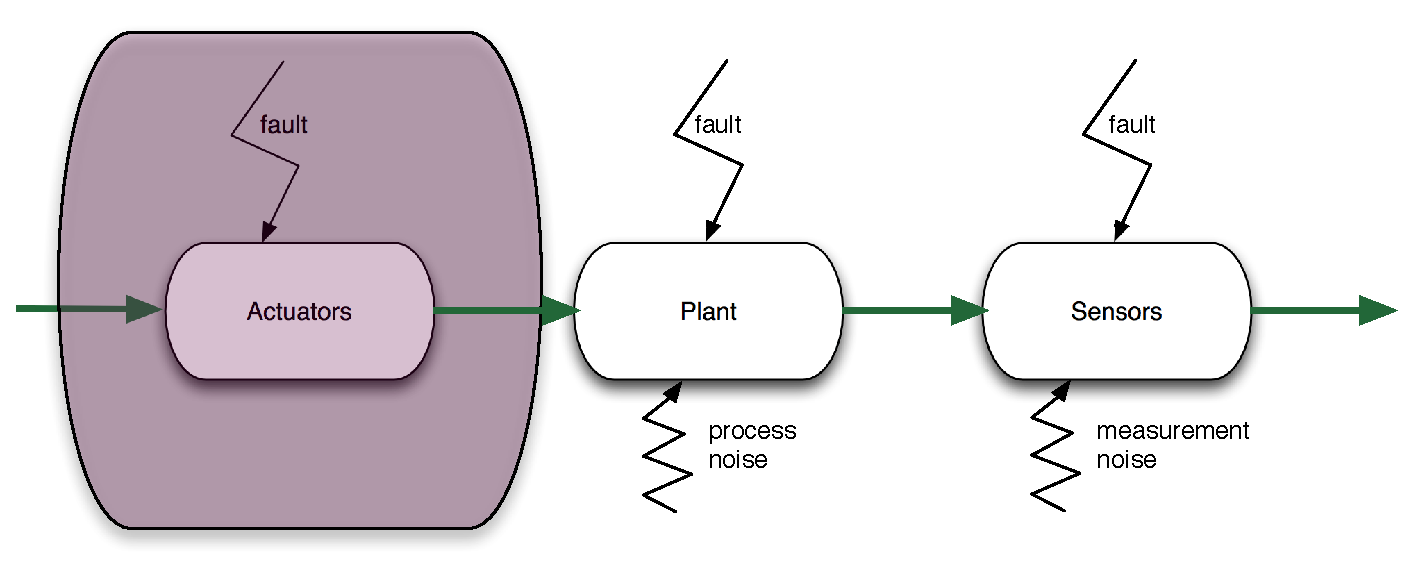
\includegraphics[width=15cm]{figures/faultsInTheSystem}    % The printed column width is 8.4 cm.
\caption{Faults altering the system } 
\label{fig:faultsInTheSystem}
\end{center}
\end{figure}

Since fault tolerant control is comprised of a set of different disciplines and is a relatively new topic, the terminology is not really established. 
FDI could be a proper example to this ambiguity. 
In some works, it stands for Fault Detection and Isolation while in some other Fault Detection and Identification, which could also named after Fault Detection and Diagnosis, 
meaning that identification is added to Fault Detection and Isolation \cite{zhang2008bibliographical}.

One of the first attempts to unify the terminology is carried out by IFAC SAFEPROCESS technical committee in 1996 and published by \cite{isermann1997trends}. 
Fault, failure, and the methodology to handle those, such as fault detection, fault isolation, fault identification, fault diagnosis and supervision terms explained separately to avoid the ongoing ambiguity 
in this field. 
Although fault detection methods are clearer, difference between the methods for two steps of fault diagnosis, namely the fault isolation and fault identification is not very obvious.

\subsection{Conventions for a Safe Flight}\label{ch2:conventions}

The widely used method to increase reliability is to use more reliable components and/or hardware redundancy. 
Both requires an increase in the cost of the UAS.
\cite{angelov2012sense}. To offer solutions for all different foreseen categories of 
airspace, a variety of approaches should be considered. While hardware redundancy 
could cope with the failure situations of UAVs in the certified airspace, it may not be 
suitable for UAVs in open or some subsets of specific categories due to budget 
constraints. Analytical redundancy is another solution, but it may be not as effective and 
simple as hardware redundancy, and it relies on the design of intelligent methods to 
utilize every bit of information onboard aircraft wisely to deal with the instances.  

There are three approaches to achieve safe FTC in standard flight conventions. 
The first one is the fail operational systems which are made insensitive to any single 
point component failure. The second approach is the fail safe systems where a 
controlled shut down to a safe state is practiced whenever a critical fault is pointed 
out by a sensor. The level of degradation ensures to switch to robust (alternate) or 
direct (minimal level of stability augmentation independent of the nature of the fault) mode. 
Switching from nominal mode to the robust and direct modes leads to a decrease 
in the available GNC functions. This causes a degradation in ease of piloting. Furthermore, some optimality conditions could have been compromised. The third approach 
is fault tolerant control systems in which redundancy in the plant and the automation 
system is used to design software that monitors the components and takes in 
actions whenever needed. The strategy is most probably to try to keep plant availability 
and to accept reduced performance \cite{blanke2000fault}.

RECONFIGURE project of FP7 \cite{goupil2015overview} aims to address at this 
problem of piloting degradation and optimality compromise by Flight Parameter Estimation (FPE) which is the online estimation of aircraft parameters, FDD and FTC in case of off-nominal events \cite{RECONFIGURE}.
They utilize a black box nonlinear model of aircraft and the project uses some outputs of a previous FP 7 project ADDSAFE leaded by Deimos Space \cite{ADDSAFE}.

\subsection{Methods for Fault Tolerant Control Systems}\label{ch1:methodsFTCS}

Among different categorizations of the fault tolerance, there are options to handle 
faults on-line or off-line. Employing fault diagnosis schemes on-line is a way to 
achieve fault tolerance. In this case, as soon as a fault is detected, a supervisory 
agent is informed via a discrete event signal. Then, accommodation of the faults 
are handled either with the selection of a predetermined controller for the specific 
fault case, or by designing the action online with real-time analysis and optimization \cite{blanke2000fault}.

Another common categorization of FTCS is passive and active FTCS. In passive FTCS, 
the flight controller is designed in such a way to accommodate not only the 
disturbances but also the faults. Active FTCS first distinguishes the fault via fault detection 
and diagnosis module and then switch between the designed controllers specific to the 
fault case or design a new one online \cite{angelov2012sense}. While active FTCS 
requires more tools to handle faults as seen in Fig.~\ref{fig:FTCS}, for faults 
not predicted and not counted for during the design of the robust controller, this method 
most probably fails. 

\begin{figure}
\begin{center}
%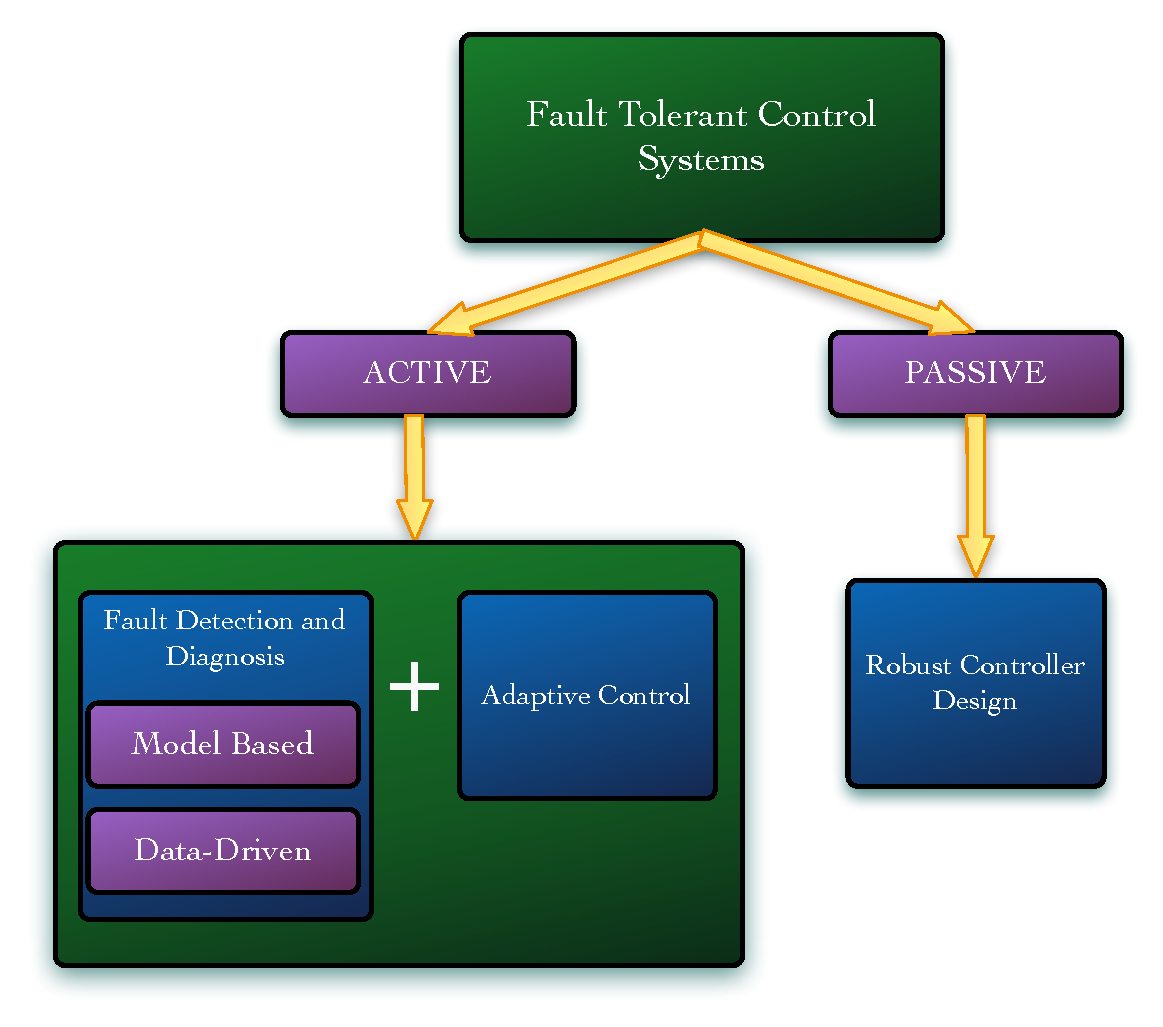
\includegraphics[width=11.3cm]{figures/FTCmethods}    % The printed column width is 8.4 cm.
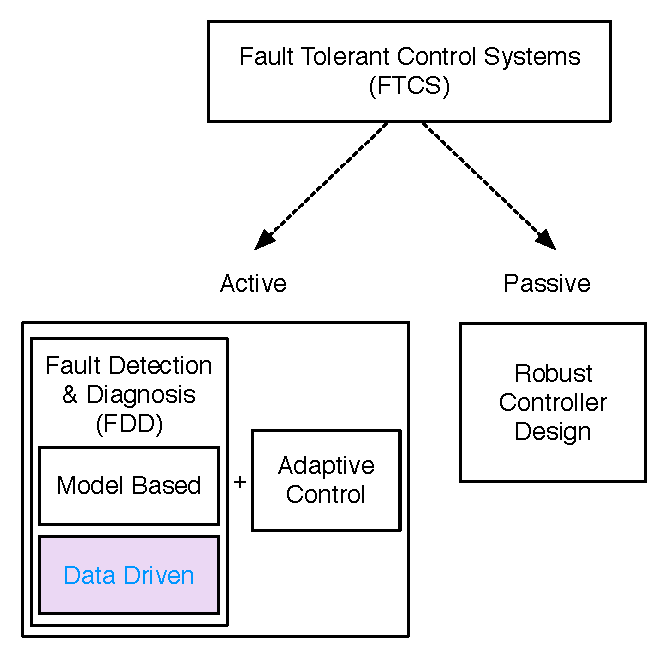
\includegraphics[width=11.3cm]{figures/FTCS}
\caption{Variations of fault tolerant control systems } 
\label{fig:FTCS}
\end{center}
\end{figure}


Even with a long list of available methods, aerospace industry has not implemented 
FTC widely, except for some space systems, because of the evolving nature of the methods, 
the tricks coming with the nonlinear nature of the problem, design complexity and high 
possibility of wrong alarms in case of large disturbances and/or modeling uncertainties. 
So, the hardware redundancy is now the preferred way because of its ease and maturity being implemented on various critical missions with human lives.

\subsection{Fault Detection and Diagnosis}

FDD is handled in two main steps; fault detection and fault diagnosis. Fault diagnosis 
encapsulates fault isolation and fault identification. FDD should 
not only be sensitive to faults but also must be robust to the model uncertainties and 
external disturbances.

Two distinct options to proceed in analytical redundancy are the model based 
approaches and data-driven approaches.
Model based fault diagnosis highlights the components of a system and the connections 
in-between, and their corresponding fault modes. 
Data driven fault diagnosis rely on the observational data and it prefers dense, redundant data with a frequency larger than the failure rate. 

% This is an example of how you would use tgrind to include an example
% of source code; it is commented out in this template since the code
% example file does not exist.  To use it, you need to remove the '%' on the
% beginning of the line, and insert your own information in the call.
%
%\tagrind[htbp]{code/pmn.s.tex}{Post Multiply Normalization}{opt:pmn}

\subsubsection{Model Based Methods}

In model based approaches, relations between measurements and estimated 
states are exploited to detect possible dysfunctions. The most common ways to 
implement a model based approach is to estimate the states, estimate the model 
parameters, or parity-space. The accuracy of the results depends on the type of 
faults (additive or multiplicative). Additive faults affects the variables of the process 
by a summation whereas the multiplicative faults by a multiplication.  When only 
output signal can be measured, signal model based methods can be used for 
fault detection such as Bandpass filters, Spectral analysis(FFT) and maximum entropy estimation. 
For the case where both the input and output signals are available, the methods used 
for fault detection are called process based methods such as: State and output 
observers(estimators), Parity equations and Identification and parameter estimation. 
They generate residuals for state variables or output variables. 
The most widely used technique for sensor and actuator faults is the state and output observers (estimators) and for process faults, identification and parameter estimation \cite{isermann1997trends}.

The output of the model based fault detection methods is the stochastic behavior 
with mean values and variances. With the use of change detection methods, deviations 
from the normal behavior can be detected. For that purpose, three available methods 
considered are, mean and variance estimation, likelihood-ratio-test and Bayes decision, 
run-sum test and two-probe t-test. Fault detection is only supported by simple threshold 
logic or hypothesis testing in most of the applications \cite{isermann1997trends}.

There are a variety of different approaches for model-based fault detection and diagnosis in the literature.
Detecting sensor and actuator faults via state estimation, utilizing an EKF is applied to a 
F-16 model in \cite{hajiyev2005sensor}. Parameter identification via $H_{\infty}$ filter 
is used to indicate icing in \cite{melody2001h}.
Another method to detect and isolate actuator/sensor faults is the multiple model adaptive estimation (MMAE) method \cite{ducard2009fault}. In MMAE \cite{magill1965optimal}, multiple Kalman filters are used as shown in Fig.~\ref{fig:mmaeScheme}. In this method, each Kalman filter $k$ uses a different system model to calculate the state estimates $\hat{x}_k$. This multiple Kalman Filters can be run in parallel, since each filter $k$ is not dependent on other Kalman Filters. The difference between the predicted measurements (calculated using the estimated states) and the real measurements $z$, gives the residual $r_k$. Residuals are used in the hypothesis conditional probability computation since they represent each model's closeness to the real model. Finally, the conditional probability $p_k$ for each model $k$ is calculated. Then, based on the conditional probabilities, state estimates are blended through a probability weighted average, that results in the final state estimate  $\hat{x}$ \cite{miller1998modified}.

\begin{figure}
\begin{center}
%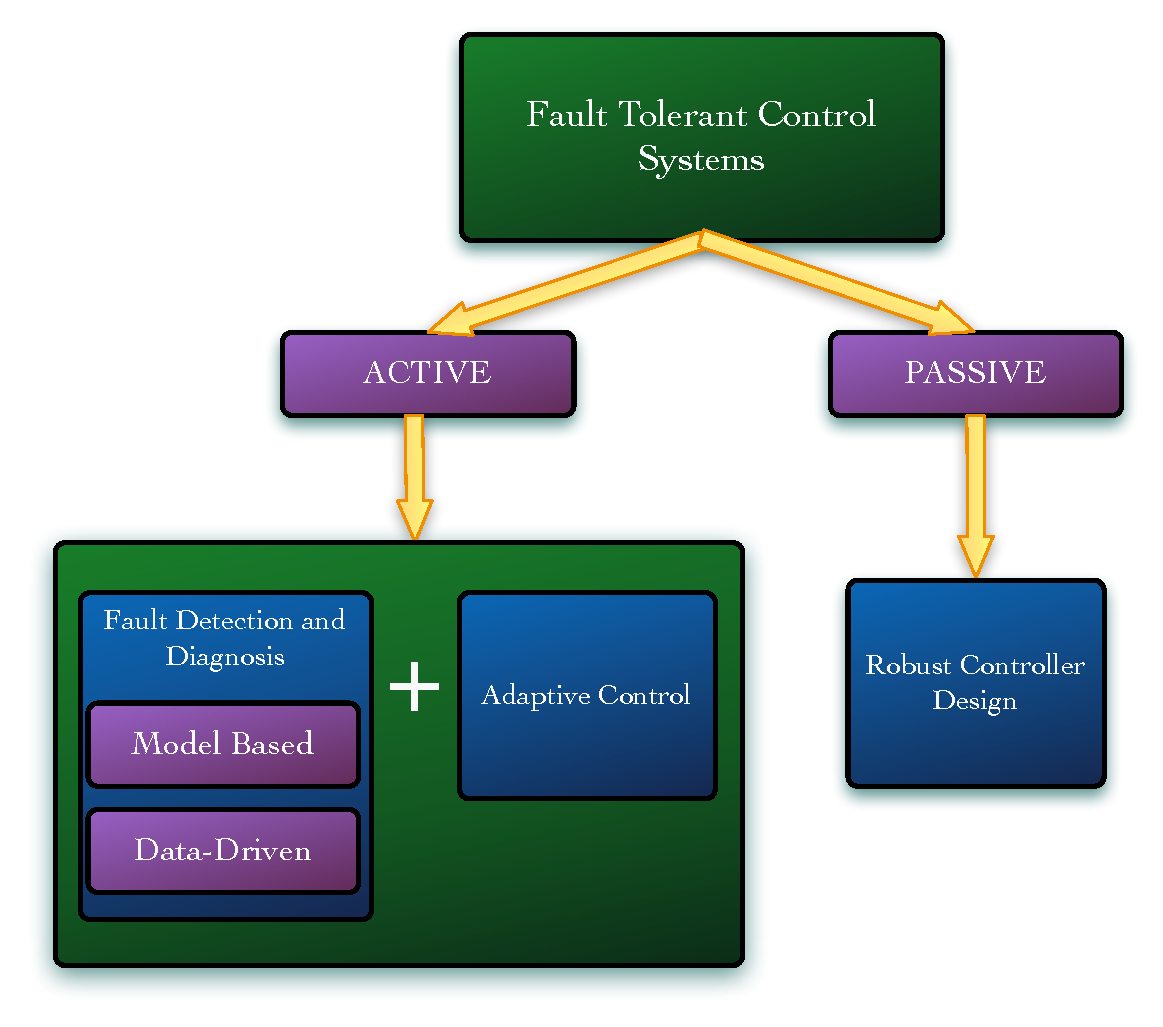
\includegraphics[width=11.3cm]{figures/FTCmethods}    % The printed column width is 8.4 cm.
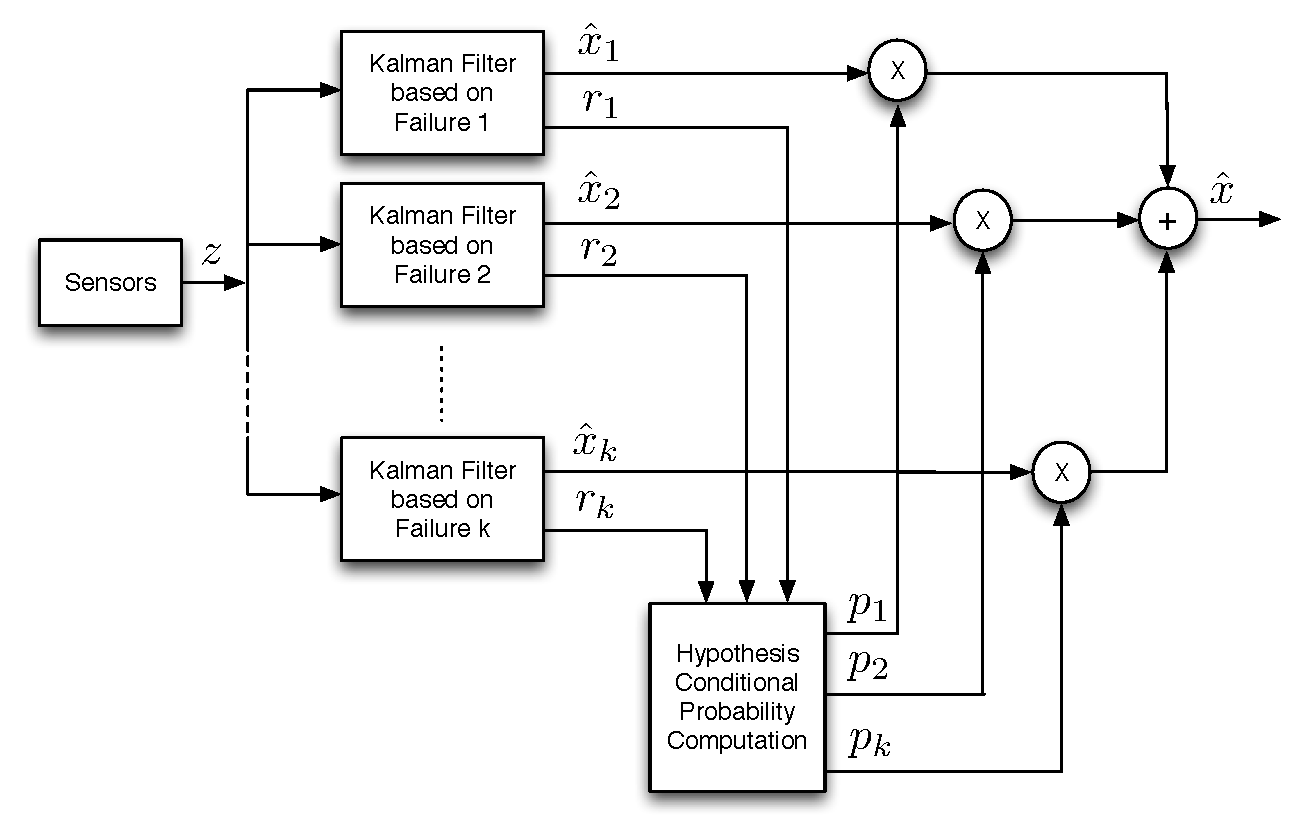
\includegraphics[width=14.7cm]{figures/mmaeScheme}
\caption{Multiple model adaptive estimation algorithm \cite{miller1998modified}} 
\label{fig:mmaeScheme}
\end{center}
\end{figure}

A drawback of model-based approaches is that they require accurate model of the 
aircraft for successful detection. In a small UAV system, which is susceptible to various 
uncertainties/disturbances and usually lacks an accurate model, using a model-based approach might fail. 
Furthermore, a mathematical model of a UAV 
is built within the flight envelope, and does not necessarily describe the 
possible dynamics invoked by a failure on-board. 

A fairly old study in 1984, investigates the design problem FDI systems robust to 
uncertainties within the models. One of the two steps of FDI (residual generation and decision-making) is targeted. They offer to handle model 
uncertainties, by designing a robust residual generation process \cite{chow1984analytical}. 
Another study deals with model uncertainties by determining the threshold of the residual 
in a novel way with an application to detect aileron actuator fault \cite{rotstein2006fault}. 
\cite{sharma2007fault} uses two cascade sliding mode observers state estimation and 
fault detection to guarantee staying in sliding manifold in the presence of unknown 
disturbances and faults. 
% This is an example of how you would use tgrind to include an example
% of source code; it is commented out in this template since the code
% example file does not exist.  To use it, you need to remove the '%' on the
% beginning of the line, and insert your own information in the call.
%
%\tgrind[htbp]{code/be.s.tex}{Block Exponent}{opt:be}

\subsubsection{Data-Driven Methods}

Model-based approaches had various successful applications until now, 
most of them assuming accurate model are available on-board. With the new 
era of UAVs, the airspace is expected to be populated by strong increase 
in the number of UAVs. The variety of UAVs, expense of accurate modeling 
practices, the difficulty in modeling the behavior of UAV in case of failures, 
call for alternative approaches for the quite challenging problem of FDD. 
The increased efficiency of on-board sensors, the increase in the computational 
capabilities of autopilot processors, and the advances in machine learning 
techniques in the last decade may offer efficient data-driven solutions to FDD.

In data driven methods, a detailed knowledge about the internal dynamics 
of the system is not necessary. The data available is the source of information 
with regard to the behavior of the system. Supervised learning, which requires 
to label the fault cases previously in the training data, is usually used for 
data-centric fault detection. In case of an unlabeled fault, the result is 
expected as a probability distribution of the available normal modes, identified 
fault labels and a probable unknown fault. What is needed at that point is to 
first detect and localize the fault and then, to consult domain experts for labeling 
for further integration of this fault into the diagnosis scheme \cite{dataCentricDiagOffline}.

\cite{gui2002fault} argues artificial intelligent methods for fault detection of complex 
systems. Comparison between Principle Component Analysis (PCA) and model based stochastic parity space 
approaches is given in \cite{hagenblad2004comparison}.
In \cite{li2016data}, the authors argues to use dynamic PCA since UAV flight 
controls is a dynamic system itself and Dynamic Principle Component Analysis (DPCA) can reflect unknown disturbances, 
while model-based approaches can only model typical disturbance.  

\section{Machines on the Rise}

Since machine learning methods are selected to detect and diagnose actuator faults in this thesis, a short introduction to the topic is given in this section. 

The mathematical analysis of learning processes goes back to 1960s when F. Rosenblatt \cite{rosenblatt1958perceptron} suggested the \emph{perceptron}: the first learning machine \cite{vapnik2013nature} (see Fig.~\ref{fig:perceptron}). 
Inspired by a simplified model of a biological neuron, the idea of perceptron was discussed for many years in neurophysiological literature \cite{vapnik2013nature}. The contribution of Rosenblatt were: to describe the perceptron model as a program for computers and to show that the model could be generalized via experiments \cite{vapnik2013nature}.
The perceptron has first been implemented on a IBM 704 as an algorithm. 
Later, a custom-built hardware implementation of the perceptron was delivered (as shown in Fig.~\ref{fig:Mark_I_perceptron}).

\begin{figure}
\begin{center}
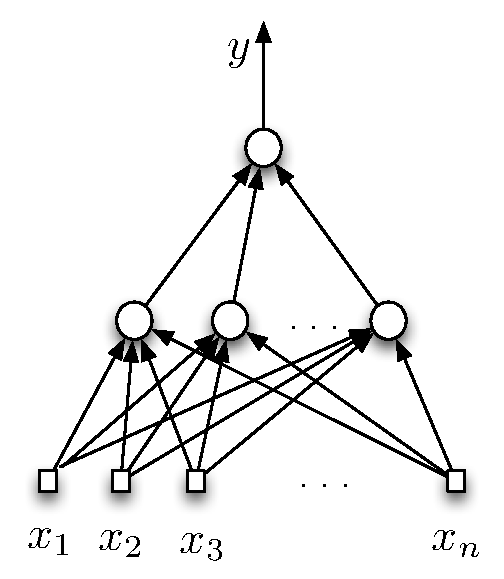
\includegraphics[width=6.1cm]{figures/perceptron}
\caption{Schematics of perceptron. The perceptron is a composition of several neurons \cite{vapnik2013nature}. $x_1$ to $x_n$ are the features and $y$ is the output.} 
\label{fig:perceptron}
\end{center}
\end{figure}

The interest in perceptron came to a halt when Minsky and Papert proved that a single layer perceptron can not learn an XOR function \cite{minsky1969perceptron}.
It led to a wrong assumption that multi-layer networks would not be able produce an XOR function. Although Grossberg published about multi-layer perceptrons capable of producing XOR functions, the declined interest has necessitated some years to pass, until the research on perceptron revived.


\begin{figure}
\begin{center}
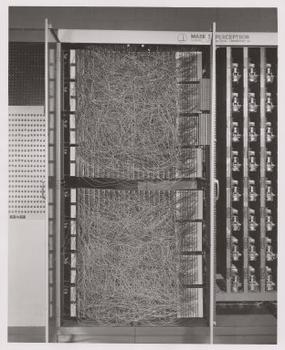
\includegraphics[width=8.3cm]{figures/Mark_I_perceptron}
\caption{Mark 1 perceptron: the first custom - built hardware implementation of the \emph{perceptron}. It is designed for image recognition with an array of 400 photocells which are connected to the "neurons" randomly.  Potentiometers are used to encode the weights, and electric motors updated the weights during learning \cite{bishop2006pattern}} 
\label{fig:Mark_I_perceptron}
\end{center}
\end{figure}

\emph{Back-propagation method}, proposed by several authors \cite{le1986learning,rumelhart1986learning} independently in 1986, is considered as the second birth of the perceptron. It is originally an older method (1963) \cite{bryson1963optimal} and used in solving control problems \cite{vapnik2013nature}. Application of the method to calculate the weight simultaneously for many neurons changed the history of learning machines \cite{vapnik2013nature}. In 80s, the terminology was also changed due to an application oriented approach in research on learning (with the introduction of powerful computers) \cite{vapnik2013nature} and multi-layer perceptrons were renamed as neural networks.

Although 1974-1980 was not very fruitful for neural networks and known as AI winter, development of statistical learning theory endured.  A novel inductive principle, \emph{Structural Risk Minimization (SRM) inductive principle}, is introduced in 1974 \cite{vapnik1974theory}. 
In SRM inductive principle, the risk in a given set of functions is minimized by controlling two factors: the value of the empirical risk and the value of the confidence interval \cite{vapnik2013nature}. 

Support Vector Machines \cite{vapnik1974theory,vapnik2006estimation} are introduced as an application of SRM by keeping the value of the empirical risk fixed (say equal to zero) and minimizing the confidence interval \cite{vapnik2013nature} as opposed to keeping the confidence interval fixed (by choosing an appropriate construction of machine) and minimizing the empirical risk (as in Neural Networks). 
Their applicability expanded thanks to its extension for problems that require nonlinear classifiers \cite{boser1992training} using \emph{kernel trick} \cite{aizerman1964theoretical} and also for problems with non-separable classes \cite{cortes1995support} using \emph{soft margin separating hyperplanes}. 


Almost 2 decades after IBM's Deep Blue beating the chess champion Kasparov \cite{deepBlue}, Google DeepMind's Artificial Intelligence(AI) AlphaGo \cite{alphaGoDeepMind,alphaGo} defeating 9-dan Go professional raises the question: what will be the next victory of AI?
European Parliament published a draft report with recommendations to the European Commission on Civil Law Rules on Robotics \cite{delvaux2017report}, including a list of concerns for a possible rise of the machines. 
Not only the singularity, artificial super intelligence resulting in deep changes in human civilization, but also more inevitable outcomes are discussed, such as AI's effects on workforce, ethical and legal issues inherent to automatized systems including drones.

\iffalse
Autonomy's effects on workforce has already been experienced, but what will be the consequences of adding more intelligence to existing automation? 
Some researchers say that, this will not lead to unemployment, but to the creation of new unforeseeable career fields, as had been the case for computer scientists after the invention of computers. 
If this is not the case, Europe is asking for solutions to cope with the imminent situation.
Until now, machine's learning processes are initiated by humans at least by giving the machine its goal. 
The community, confident that the robots will not evolve to some sort of consciousness, is referring to this fact, robots will always need humans to provide them with objectives. 
While this is debated, Google is discussing to implement a big red button to its AI DeepMind, just in case. 
The European Parliament also advices AI designers to integrate kill switches to AI. 
However, according to some experts, if an AI becomes smart enough, it might disable the kill switch and avoid such interruption. 
Although this sounds like science fiction, here we are, referencing to Isaac Asimov's laws\footnote{1. A robot may not injure a human being or, through inaction, allow a human being to come to harm. 2. A robot must obey the orders given it by human beings except where such orders would conflict with the First Law. 3. A robot must protect its own existence as long as such protection does not conflict with the First or Second Laws \cite{asimovLaws} 0. A robot may not harm humanity, or, by inaction, allow humanity to come to harm.} in documents by European Parliament \cite{civilLawRulesOnRobotics}.

Douglas Hofstadter, in his book \emph{Godel Escher Bach - An Eternal Golden Braid}, makes two analogies between: unconscious things and meaningless symbols; consciousness and patterns that are made up of these meaningless symbols \cite{hofstadter1980godel}. 
If he is right, witnessing the AI's powers in recognizing patterns, consciousness might a probable outcome in the future. 
Concerns from the European Parliament is shared by popular scientists and investors such as Elon Musk \cite{AIthreatEMusk}, Bill Gates \cite{AIthreatBGates} and Stephen Hawking \cite{AIthreatSHawking}. Watching Google's humanoid robot, Atlas, running freely in the woods does not help to relieve. Opposed to the idea of this powerful tool dominated by a company or a nation, OpenAI, a nonprofit company, is aiming to distribute AI knowledge publishing open source code \cite{openAI}. Broad share of AI is also underlined in the document by European Parliament, with the proper regulations expected in the years to come.
Until then, as suggested by European Parliament, we will refer to Asimov's Laws while designing AI.


With the last turn in popularity and practicality contest among research topics of the last decade, machine learning and drones seem to be neck to neck. The sides of the race are mostly supported by high tech rather than the public who has concerns in both opponents. Is there a chance that these two can run side by side with cheers? Machine learning guides various aspects of our lives even without noticing it due to its abrupt introduction via the bigger tech companies. Its abilities rise, defeating 9-dan Go professional, their accuracy increase, enabling smooth voice recognition, adding intelligence to our daily lives. Another machine, who wants to enjoy this enabling technology is a drone. Drones, although still very strictly regulated in most countries have been spreading with great passion along their enthusiasts. 
\fi

The winner of the Go contest, the AI, is based on a method named \emph{Reinforcement Learning} (RL). This method is used in many of the latest exciting applications of AI. In reinforcement learning, the selection of actions results in consequences. Thus, the agent interacts with its environment, by taking actions and observing the consequences via the reward function. The goal of the agent is the calculate actions that will maximize the reward. An example to this functioning can be demonstrated on a robot locomotion problem. Fig.~\ref{fig:deepmindWalking} shows a humanoid model and an ant robot model from \emph{Google DeepMind} \cite{deepmindWebsiteHumonoidWalking,deepmindHumonoidWalkingStanford,deepmindHumonoidWalkingVideo}. The robot models have virtual sensors which give information about their states (angle and position of the joints \cite{deepmindHumonoidWalkingStanford}) and surrounding objects \cite{deepmindHumonoidWalkingVideo}. The objective of the robots are to go from point A to point B. Although the robots are not explicitly programmed to walk or jump, or not given any information about what walking or jumping looks like, they learnt to move very similar to walking and jumping.


\begin{figure}
\begin{center}
%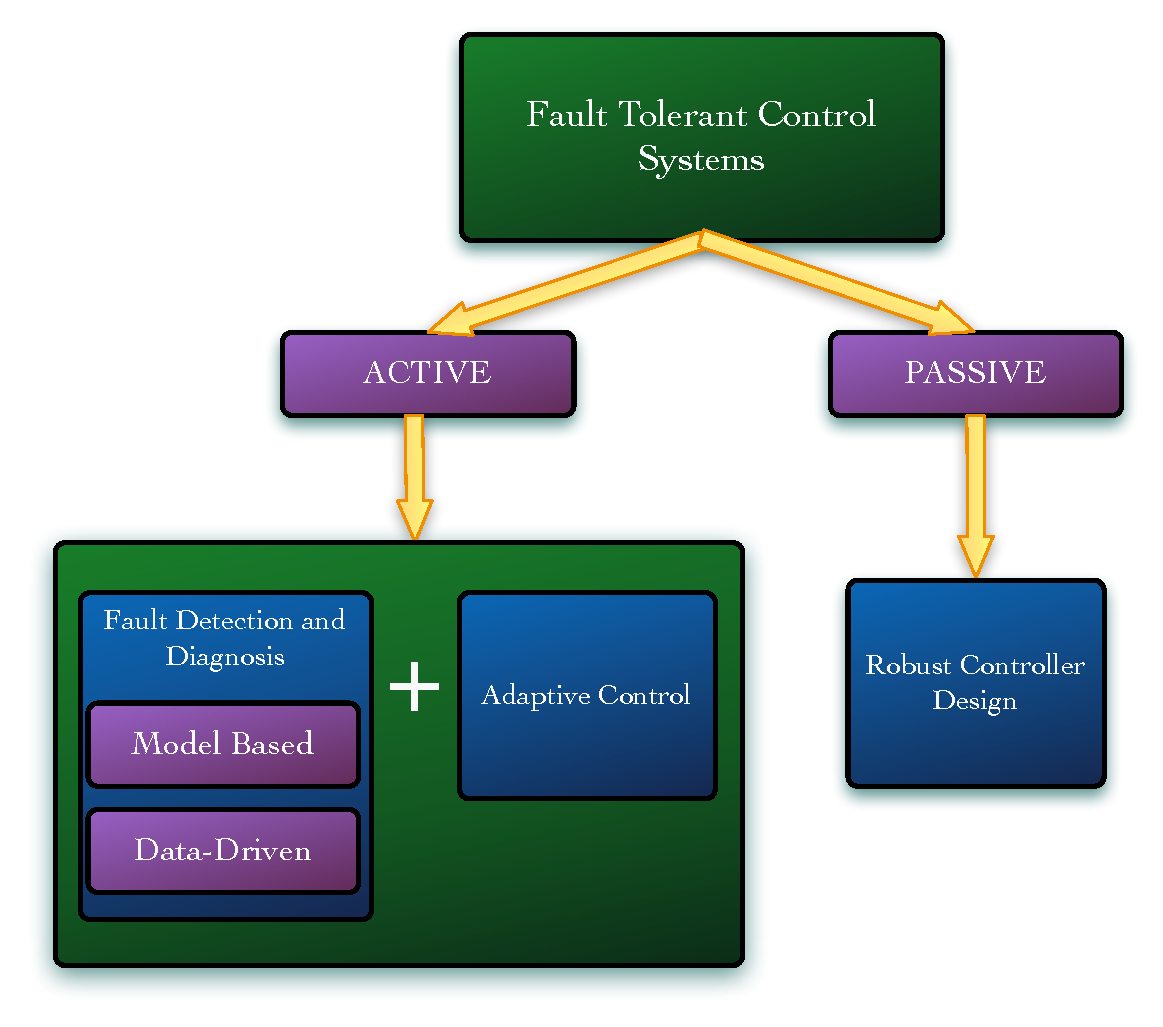
\includegraphics[width=11.3cm]{figures/FTCmethods}    % The printed column width is 8.4 cm.
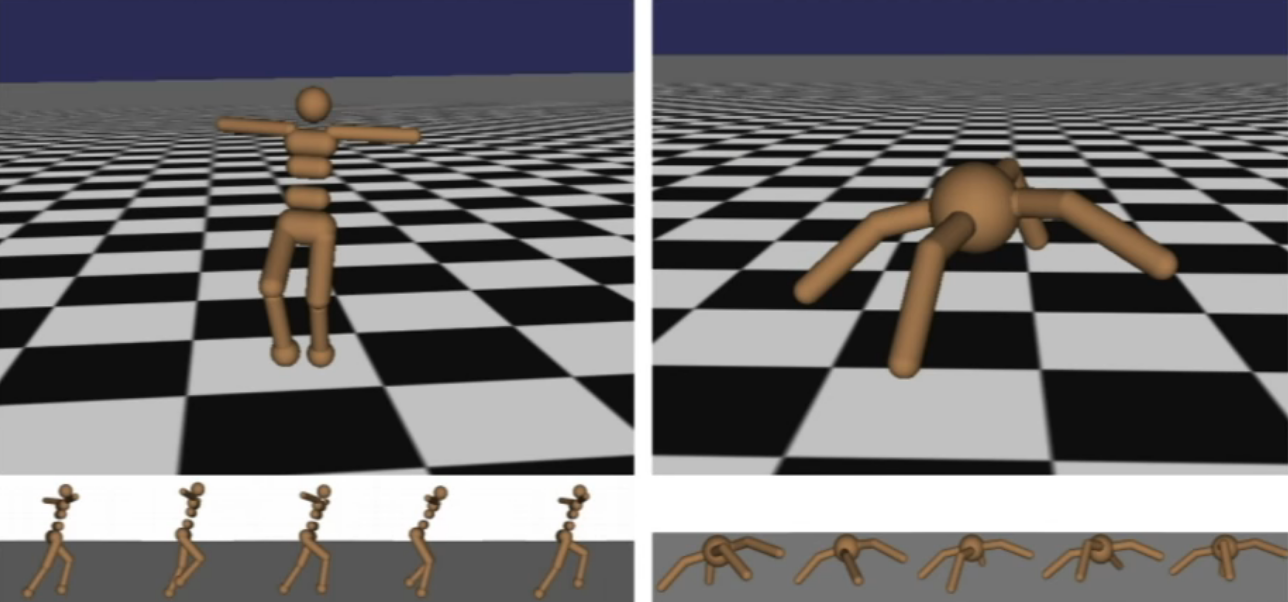
\includegraphics[width=13.3cm]{figures/deepmindWalking}
\caption{Humanoid and ant robot models \cite{deepmindHumonoidWalkingStanford} exhibiting walking and jumping motions respectively using reinforcement learning \cite{deepmindWebsiteHumonoidWalking}. The robots are given objectives to go from one point to the other, but not given any information about walking or jumping \cite{deepmindHumonoidWalkingVideo}.} 
\label{fig:deepmindWalking}
\end{center}
\end{figure}

We witness very promising application results in Neural Networks and its varieties lately. Convolutional neural networks (CNN) applied to image processing problems, and sequence models (Recurrent Neural Networks (RNN and Long short term memory (LSTM) ) applied to natural language processing produced incredible results raising the interest in machine learning and AI in various fields. Such an example is Google's \emph{Duplex} AI \cite{googleDuplex}, making phone calls to restaurants or hair dresser's, to book a table or take a rendezvous.  AI talks to the person on the phone and adapts to the responses of the human on the phone, and achieves its task without being exposed that it is actually an AI.



\begin{figure}
\begin{center}
%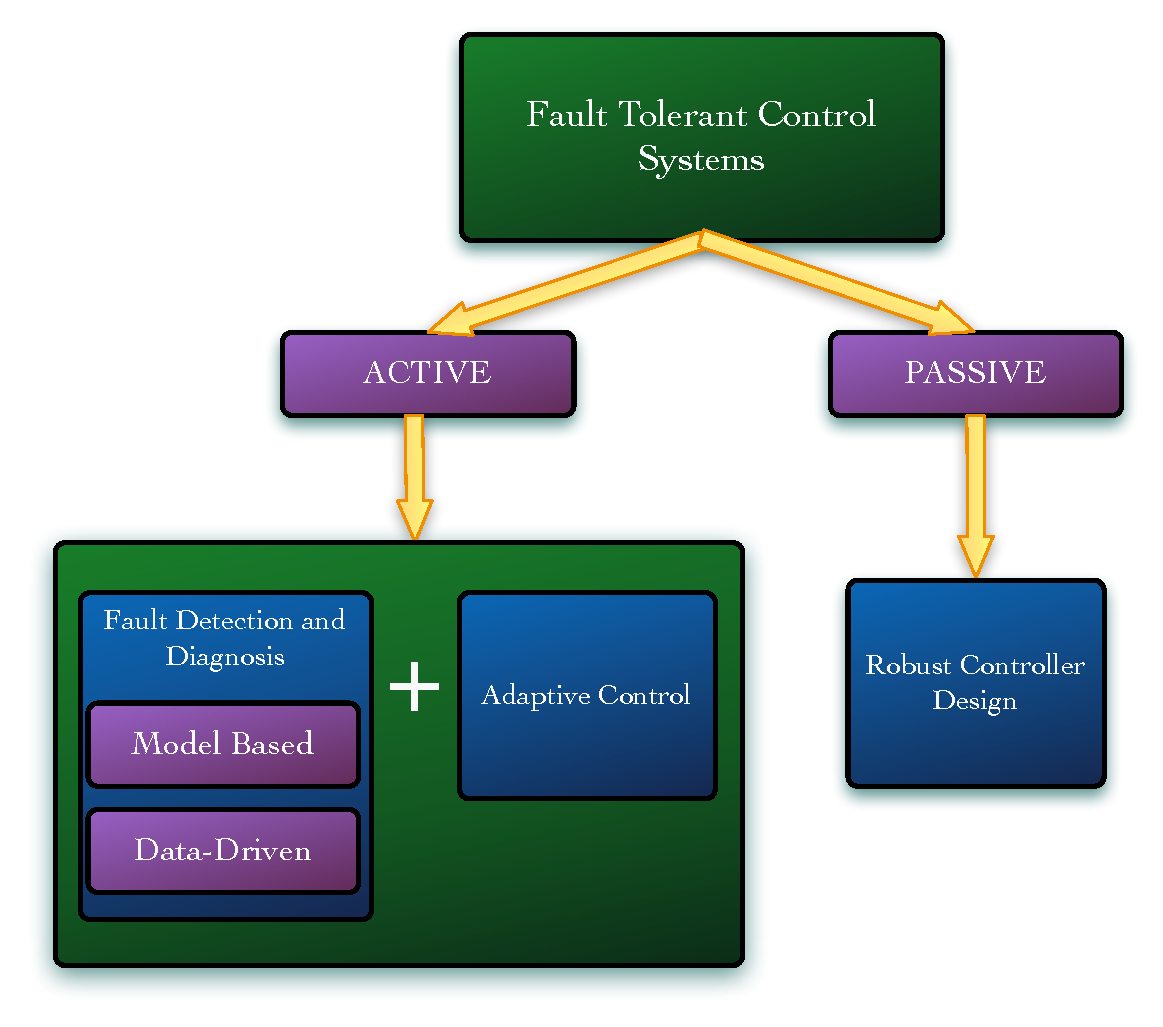
\includegraphics[width=11.3cm]{figures/FTCmethods}    % The printed column width is 8.4 cm.
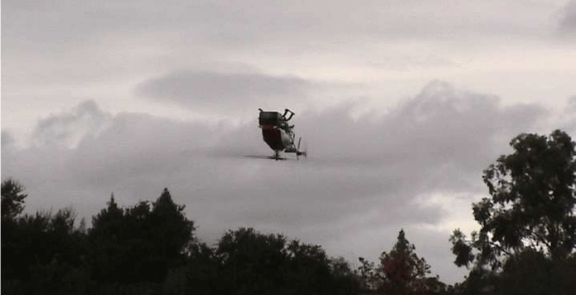
\includegraphics[width=13.1cm]{figures/invertedHelicopterAndrewNg}
\caption{Autonomous helicopter from Stanford University learns to fly acrobatic maneuvers using RL in autopilot \cite{ng2003shaping}} 
\label{fig:invertedHelicopterAndrewNg}
\end{center}
\end{figure}

An application of RL in aviation is demonstrated on Stanford University's autonomous helicopter \cite{ng2003shaping}. Thanks to RL, the helicopter's autopilot performs acrobatic maneuvers, which is quite difficult to do with a hardcoded controller design. A photo taken during its inverted flight can be seen in Fig.~\ref{fig:invertedHelicopterAndrewNg}.


Machine learning has already started to take part in aviation. Operational improvements on aviation is one of the preliminary fields it appeared. Recently, in an AGE sponsored competition, data scientists designed a routing algorithm using real flight data, and achieved 12\% improvement in fuel consumption efficiency. Some other operational problems issued by machine learning are accurate arrival time estimation and calculating optimal parameters for take off, mostly for reducing the airline costs and increasing customer satisfaction. Yet another application is to deal with the expected shortage of pilots, inevitable in the years to come, thanks to the increasing demand for air travel. So, a prospective utilization of machine learning is to assess the competency of pilots with unsupervised learning models in order to reduce the long duration of pilot training, hence contributing to tackle pilot shortage problem. Use of data-driven approaches for pilot training could be used not only for assessment of the pilots but also to increase the efficiency of the training by offering trainee focused personal training, adapting the curriculum to their individual skills and needs. To overcome the pilot shortage, another way to handle the problem might be to reduce the need for one. 

AI has actually already sneaked into the cockpit. Garmin implemented voice recognition features garnished with some other functions such as changing radio channels to aid the pilots with its audio panels GMA 350 and GMA 35, called \emph{Telligence}. 
One of the goals of the autonomy researchers is to look for ways to implement artificial intelligence to one of the core features of an aircraft: the autopilot. Hence the ability to use them is tricky due to the inherent nature of the methods, non-determinism. EASA A-NPAs offer different categories to enjoy for drones, depending on the risk of the operation of concern. The difficulties waiting the machine learning researches are not really well defined or widely argued in aviation. 


\section{Conclusion}

In this chapter, we have discussed the current status of drone regulations, an introduction to \emph{Paparazzi Autopilot} which is used in this thesis, the advantages of open-source systems to aid drone integration into the airspace. Then, fault tolerant control systems are introduces with a focus on fault detection and diagnosis. Two main methods, model-based and data-driven, are discussed via referring to the literature. Then, general advancements in artificial intelligence (AI) are addressed, since one of its techniques, machine learning, is used as the methodology to detect the faults in this thesis. 

Next, nonlinear aircraft dynamics will be discussed. The reason here is to give insights about flight motion, and simulate the states of an aircraft. Those states then can be used to simulate sensor measurements onboard a drone. Those measurements are necessary to design data-driven fault detection \& diagnosis algorithms.
